\documentclass[10pt]{article}

\usepackage[utf8]{inputenc}
\usepackage{tabularx}
\usepackage{hyperref}
\usepackage{array}  
\usepackage{graphicx}
\usepackage{geometry}
\usepackage{fancyhdr}
\usepackage{tikz}
\usepackage{pgf-pie}
\usepackage{anyfontsize}
\usepackage[table,xcdraw]{xcolor}
\usepackage{tabularx, etoolbox}
\usepackage{eso-pic} 
\usepackage{float}
\usepackage{setspace}
\usepackage{longtable}


\newcommand\version{2.0.0} %aggiunta versione come variabile

\graphicspath{{images/}}
%\graphicspath{{../../images/}}

%cambio misure della pagina
\geometry{a4paper,left=20mm,right=20mm,top=20mm}
\setlength{\parindent}{0pt}
%ebdfc7
\definecolor{colorePie}{HTML}{ebdfc7}

% Imposta il livello di profondità dell'indice
\setcounter{tocdepth}{4} % Aggiunge paragraph all'indice

% Abilita la numerazione fino a paragraph
\setcounter{secnumdepth}{5} % Estende la profondità della numerazione


\pagestyle{fancy}
\fancyhf{}
\renewcommand{\headrulewidth}{0.4pt}
\lhead{
    \parbox[c]{1cm}{\includegraphics[width=1.1cm]{Sevenbitslogo.png}}
}
\rhead{\textcolor[HTML]{9e978a}{ Piano di Progetto v\version}
}
\setlength{\headheight}{25pt}
\cfoot{\thepage}


\renewcommand*\contentsname{Indice}
\renewcommand{\listfigurename}{Elenco delle figure}
\renewcommand{\listtablename}{Elenco delle tabelle}

\begin{document}

% Pagina del titolo
\begin{titlepage}
    \setcounter{page}{0}
    \centering
    % Inserisci il logo del gruppo (modifica il percorso dell'immagine)
    \includegraphics[width=7.2cm]{Sevenbitslogo.png} \\[2cm] 
    
    % Titolo
     {\fontsize{40}{40}\bfseries Piano di Progetto}\selectfont \\[3.9em]
    
    % Sottotitolo
    % Email del gruppo
    {\large sevenbits.swe.unipd@gmail.com} \\[3em]
    
    % Spazio per il logo dell'università
    \hfill
     
    \AddToShipoutPictureBG{ % Imposta il triangolo con logo
        \ifnum\value{page}=0
        \begin{tikzpicture}[overlay]
        
            % Definisce un triangolo blu in basso a destra
            \fill[colorePie] 
                (current page.south east) -- ++(-9cm,0) -- ++(9cm,9cm);
            
            % Inserisce il logo all'interno del triangolo
            \node[anchor=south east, xshift=-0.3cm, yshift=0.3cm] at (current page.south east) {
                \includegraphics[width=4.5cm]{LogoUnipd.png}
            };
        \end{tikzpicture}
        \fi
    }

\vfill
\end{titlepage}
\newpage
\clearpage

\setcounter{page}{1}
%registro modifiche
\begin{center}
\textbf{Registro modifiche}\\
\vspace{2mm}
\renewcommand{\arraystretch}{1.5}
\rowcolors{0}{gray!11}{white} % Aggiunge colore alle righe del registro

\begin{longtable}{|>{\centering\arraybackslash}m{1.5cm}|>{\centering\arraybackslash}m{2cm}|>{\centering\arraybackslash}m{2.5cm}|>{\centering\arraybackslash}m{2.5cm}|>{\centering\arraybackslash}m{5cm}|}
\hline
\textbf{Versione} & \textbf{Data} & \textbf{Autore} & \textbf{Verificatore} & \textbf{Descrizione}\\
\endhead
\hline
2.0.0 & 2025-04-10 & Leonardo Trolese & Manuel Gusella & Approvazione documento per PB$_G$\\
\hline
1.0.6 & 2025-04-10 & Leonardo Trolese & Manuel Gusella & Fine redazione undicesimo sprint$_G$ \ref{undicesimo-sprint}\\
\hline 
1.0.5 & 2025-04-04 & Leonardo Trolese & Manuel Gusella & Inizio redazione undicesimo sprint$_G$ \ref{undicesimo-sprint}\\
\hline 
1.0.4 & 2025-03-28 & Uncas Peruzzi & Federico Pivetta & Redazione decimo sprint$_G$ \ref{decimo-sprint}\\
\hline
1.0.3 & 2025-03-21 & Federico Pivetta & Uncas Peruzzi & Redazione nono sprint$_G$ \ref{nono-sprint}\\
\hline
1.0.2 & 2025-03-17 & Riccardo Piva & Alfredo Rubino & Redazione ottavo sprint$_G$ \ref{ottavo-sprint}\\
\hline
1.0.1 & 2025-03-08 & Giovanni Cristellon & Leonardo Trolese & Redazione settimo sprint$_G$ \ref{settimo-sprint}\\
\hline
1.0.0 & 2025-02-21 & Giovanni Cristellon & Manuel Gusella & Approvazione documento per RTB$_G$.\\
\hline
0.4.9 & 2025-02-21 & Alfredo Rubino & Manuel Gusella & Modifica colori tabelle\\
\hline
0.4.8 & 2025-02-20 & Alfredo Rubino & Giovanni Cristellon & Redazione sesto sprint$_G$ \ref{sesto-sprint} e correzioni quinto sprint$_G$ \ref{quinto-sprint}\\
\hline
0.4.7 & 2025-02-06 & Riccardo Piva & Federico Pivetta & Piccole correzioni quinto sprint$_G$ \ref{quinto-sprint}\\
\hline
0.4.6 & 2025-01-29 & Riccardo Piva & Federico Pivetta & Redazione quinto sprint$_G$ \ref{quinto-sprint}\\
\hline
0.4.5 & 2025-01-11 & Leonardo Trolese & Peruzzi Uncas & Redazione quarto sprint$_G$ \ref{quarto-sprint}\\
\hline
0.4.4 & 2024-12-19 & Federico Pivetta & Peruzzi Uncas & Redazione terzo sprint$_G$ \ref{terzo-sprint}\\
\hline
0.4.3 & 2024-12-11 & Peruzzi Uncas & Alfredo Rubino & Redazione secondo sprint$_G$ \ref{secondo-sprint}\\
\hline
0.4.2 & 2024-12-10 & Peruzzi Uncas & Alfredo Rubino & Refactoring stile analisi rischi e aggiunta sezione identificazione\\
\hline
0.4.1 & 2024-12-10 & Federico Pivetta & Alfredo Rubino & Aggiunta di RT2, RC1, RC2, RC3, RP1 e RP2\\
\hline
0.4.0 & 2024-12-02 & Federico Pivetta & Leonardo Trolese & Stesura iniziale della sezione \ref{analisi-rischi}, completa della sottosezione \ref{introduzione-analisi} e aggiunta di RT1\\
\hline
0.3.2 & 2024-11-28 & Manuel Gusella & Giovanni Cristellon & Fine stesura primo sprint$_G$ \ref{primo-sprint} e aggiunta immagini\\
\hline
0.3.1 & 2024-11-22 & Manuel Gusella & Riccardo Piva & Stesura sottosezione \ref{struttura-espositiva}\\
\hline
0.3.0 & 2024-11-22 & Manuel Gusella & Riccardo Piva & Stesura iniziale della sezione \ref{modello-sviluppo} e sottosezioni Modello di sviluppo, preventivo e consuntivo\\
\hline
0.2.1 & 2024-11-17 & Manuel Gusella & Federico Pivetta & Modifiche di stile delle liste e dei link nel verbale \\
\hline
0.2.0 & 2024-11-15 & Manuel Gusella & Federico Pivetta & Stesura iniziale sezione \ref{pianificazione}\\
\hline
0.1.0 & 2024-11-14  & Manuel Gusella & Riccardo Piva & Stesura sezione \ref{introduzione}\\
\hline
\end{longtable}
\rowcolors{0}{}{} % Riporta le righe alla colorazione originale
\end{center}


\newpage
\tableofcontents
\newpage
\listoffigures
\newpage
\listoftables

\newpage
\section{Introduzione}
\label{introduzione}
\subsection{Scopo del documento}
Questo documento ha lo scopo di definire in modo chiaro le modalità con cui le attività saranno svolte dai membri del gruppo per la realizzazione del progetto$_G$.\\
Saranno trattati in dettaglio i seguenti temi:
\begin{itemize}
    \item [-] Analisi dei rischi;
    \item [-] Organizzazione delle attività nei singoli periodi;
    \item [-] Suddivisione dei ruoli tra i membri del gruppo;
    \item [-] Stima dei costi e delle risorse nelle varie iterazioni.
\end{itemize}

\subsection{Scopo del capitolato}
Il capitolato$_G$ C4 ha come scopo la realizzazione di una dashboard$_G$ "amministrativa" in grado di proporre ad ogni utente degli annunci personalizzati tramite l'utilizzo di LLM$_G$.\\ 
La dashboard$_G$ deve mostrare una mappa con ipotetici utenti generati virtualmente, che poi verranno rappresentati come punti in movimento, e ogni volta che un utente passa per un'area di interesse appare un annuncio generato tramite IA$_G$.

\subsection{Glossario}
Al fine di evitare ambiguità relative alla terminologia utilizzata all'interno del documento, è presente il \textit{Glossario.pdf}, in cui vengono riportate tutte le definizioni delle parole con un significato specifico. Questi termini verranno marcati con una $_G$ a pedice, mentre i termini composti, oltre alla $_G$ a pedice, saranno uniti da un "-" come segue: termine-composto$_G$. 

\subsection{Riferimenti}
\subsubsection{Informativi}
Slide del corso di Ingegneria del Software:
\begin{itemize}
\item [-] Modelli di sviluppo software:\\ \textcolor{blue}{\texttt{\url{https://www.math.unipd.it/~tullio/IS-1/2024/Dispense/T03.pdf}}}\\
(Consultato: 2025-02-19).
\item [-] Gestione di Progetto:\\ \textcolor{blue}{\texttt{\url{https://www.math.unipd.it/~tullio/IS-1/2024/Dispense/T04.pdf}}}\\
(Consultato: 2025-02-19).
\end{itemize}

\subsubsection{Normativi}
\begin{itemize}
\item [-] \textit{Norme\_di\_Progetto\_v1.0.0.pdf}
    \item [-] Documento e presentazione del capitolato C4 - NearYou - Smart custom advertising platform:\\
    \textcolor{blue}{\texttt{\url{https://www.math.unipd.it/~tullio/IS-1/2024/Progetto/C4.pdf}}}\\
(Consultato: 2025-02-19).\\
\textcolor{blue}{\texttt{\url{https://www.math.unipd.it/~tullio/IS-1/2024/Progetto/C4p.pdf}}}\\
(Consultato: 2025-02-19).
    
\item [-] Regolamento del progetto didattico\\ \textcolor{blue}{\texttt{\url{https://www.math.unipd.it/~tullio/IS-1/2024/Dispense/PD1.pdf}}}\\
(Consultato: 2025-02-19).
\end{itemize}

\newpage
\section{Analisi dei Rischi}
\label{analisi-rischi}
    \subsection{Introduzione}
    \label{introduzione-analisi}
    L'analisi dei rischi è un processo$_G$ che ha l'obiettivo di anticipare e gestire le diverse situazioni avverse che possono sorgere durante il ciclo-di-vita$_G$ di un progetto$_G$.\\
    Il gruppo, in conformità allo standard ISO/IEC 31000:2018, si è concentrato sull'identificazione, comprensione e classificazione dei rischi in base alla loro probabilità di verificarsi e alle possibili ripercussioni che ne deriverebbero.\\ 
    L'approccio adottato si può articolare in cinque fasi fondamentali:
    \begin{enumerate}
        \item \textbf{Individuazione dei Rischi}:
        Questa fase consiste nell'individuazione in maniera esaustiva di tutti gli eventi e le cause potenzialmente sfavorevoli che potrebbero verificarsi nel corso del progetto$_G$. Si raggiunge la conclusione una volta creato un elenco degli elementi che rappresentano delle minacce al raggiungimento degli obiettivi prefissati;
        \item \textbf{Analisi dei Rischi}:
        Questa fase consiste nell'analisi dettagliata di tutti i rischi e nella determinazione delle azioni da intraprendere più appropriate, con l'obiettivo di prendere decisioni corrette riguardo alle misure di attenuazione e alla gestione degli eventi;
        \item \textbf{Valutazione dei Rischi}:
        Questa fase consiste nella valutazione dei rischi in termini di probabilità di occorrenza e potenziali ripercussioni, al fine di stabilire la priorità delle misure di attenuazione per gestire al meglio ciascuna situazione avversa;
        \item \textbf{Gestione dei Rischi}:
        Questa fase consiste nell'adozione delle misure di attenuazione o prevenzione, in base alla natura e all'entità del rischio$_G$. Le decisioni prese durante la fase di Analisi dei Rischi si traducono in azioni concrete;
        \item \textbf{Monitoraggio e Revisione dei Rischi}:
        Questa fase consiste in un monitoraggio continuo dei rischi identificati, per garantire l'efficacia delle misure adottate e per rilevare tempestivamente la comparsa di nuovi rischi;
    \end{enumerate}
    I rischi identificati sono stati suddivisi in tre categorie principali:
    \begin{itemize}
        \item \textbf{Rischi Tecnologici}: Riguardano le incertezze e i possibili fallimenti legati alle tecnologie impiegate nel progetto$_G$, come malfunzionamenti o difficoltà nell'integrazione; 
        \item \textbf{Rischi di Comunicazione}: Riguardano le difficoltà nello scambio di informazioni tra i membri del gruppo o con la proponente$_G$, che potrebbero compromettere il corretto svolgimento del progetto$_G$;
        \item \textbf{Rischi di Pianificazione}: Riguardano le problematiche relative alla gestione del tempo, delle scadenze e delle risorse, inclusi eventuali ritardi, stime imprecise o spreco delle risorse;
    \end{itemize}

    \subsubsection{Struttura dei Rischi}
    Il formato utilizzato per la classificazione dei rischi è R[Tipo][Indice], dove:
    \begin{itemize}
        \item \textbf{R}: abbreviazione di "Rischio";
        \item \textbf{Tipo}: rappresenta la categoria del rischio$_G$ e può essere:
        \begin{itemize}
            \item \textbf{T}: Rischio$_G$ Tecnologico;
            \item \textbf{C}: Rischio$_G$ di Comunicazione;
            \item \textbf{P}: Rischio$_G$ di Pianificazione;
        \end{itemize}
        \item \textbf{Indice}: numero progressivo che identifica univocamente ciascun rischio$_G$ all'interno della categoria di appartenenza.
    \end{itemize}
\rowcolors{1}{white}{white}
\subsection{Rischi Tecnologici}
    {\renewcommand{\arraystretch}{1.5}%
    \subsubsection{RT1 - Complessità delle nuove tecnologie}
    \label{RT1}
    \begin{tabularx}{\textwidth}{|l|X|}
    \hline
    \rowcolor{gray!25}
    Codice & RT1 \\
    \hline
    Descrizione & Il progetto$_G$ richiede l'utilizzo di tecnologie poco conosciute o con cui il gruppo ha un'esperienza limitata. Di conseguenza l'apprendimento e l'adattamento a queste nuove tecnologie richiede del tempo, che potrebbe comportare rallentamenti nel progresso del progetto$_G$.\\
    \hline
    Identificazione & Il responsabile del progetto$_G$ deve considerare le competenze dei membri del gruppo durante l'assegnazione delle task, allo stesso tempo quest'ultimi sono tenuti ad avvisare tempestivamente il responsabile se riscontrata qualche difficoltà.  \\
    \hline
    Possibili Attenuazioni & Per affrontare la complessità delle nuove tecnologie, verranno adottate diverse strategie. L'azienda proponente$_G$ si è resa disponibile ad organizzare incontri focalizzati su tecnologie specifiche, per risolvere eventuali dubbi. Inoltre, i membri del gruppo collaboreranno attivamente, condividendo le proprie informazioni al fine di raggiungere un livello condiviso di conoscenze. Infine, verrà dedicato del tempo alla fase di apprendimento, consentendo al gruppo di esplorare diverse tecnologie, identificare i punti di forza e le criticità, così da accelerare l'apprendimento e prevenire errori futuri.\\
    \hline
    Probabilità Occorrenza & Alta \\
    \hline
    Pericolosità & Alta \\ 
    \hline
    \end{tabularx}

    
    \subsubsection{RT2 - Carenza di documentazione sulle tecnologie}
    \label{RT2}
    \begin{tabularx}{\textwidth}{|l|X|}
    \hline
    \rowcolor{gray!25}
    Codice & RT2 \\
    \hline
    Descrizione & L'apprendimento di nuove tecnologie necessarie allo sviluppo del progetto$_G$ richiede un significativo investimento di tempo. Quando queste tecnologie sono carenti di una documentazione$_G$ adeguata, il processo$_G$ di apprendimento diventa ancora più complesso e impegnativo.\\
    \hline
    Identificazione & Questa difficoltà può manifestarsi quando gli sviluppatori faticano a procedere in maniera significativa nella fase di sviluppo, il responsabile deve percepire eventuali rallentamenti o carenza di ore produttive nella rendicontazione e prendere delle decisioni.  \\
    \hline
    Possibili Attenuazioni & Una possibile soluzione consiste nell'organizzare una fase iniziale durante la quale il gruppo possa familiarizzare con la tecnologia. In questa fase, la proponente$_G$ potrebbe offrire un supporto, eventualmente coinvolgendo esperti con esperienza nella tecnologia, se disponibili. Qualora la tecnologia non risulti strettamente indispensabile per il progetto$_G$, si potrebbe considerare l'adozione di una soluzione alternativa con una documentazione$_G$ più completa.\\
    \hline
    Probabilità Occorrenza & Media \\
    \hline
    Pericolosità & Alta \\ 
    \hline
    \end{tabularx}

    \subsubsection{RT3 - Produzione di codice confuso o con errori}
    \label{RT3}
    \begin{tabularx}{\textwidth}{|l|X|}
    \hline
    \rowcolor{gray!25}
    Codice & RT3 \\
    \hline
    Descrizione & In fase di sviluppo è piuttosto plausibile la presenza di bug$_G$ nel codice o di codice non facilmente leggibile e interpretabile da un altro componente del team. Questo è dovuto all'inesperienza del team nella scrittura di codice enterprise per progetti di rilevante dimensione. \\
    \hline
    Identificazione & Un chiaro indicatore è la presenza di ripetuti colloqui tra componenti del team volti a esplicare il codice che non risulta chiaro. Per quanto riguarda la presenza di bug$_G$, può essere intercettata tramite la normale esecuzione del codice o mediante la fase di testing.   \\
    \hline
    Possibili Attenuazioni & In caso di codice poco leggibile è necessario effettuare un refactoring e continue review del software. In caso di errori, si può chiedere l'aiuto di un membro del team più esperto o organizzare delle brevi sessioni di peer-programming per risolvere il problema. \\
    \hline
    Probabilità Occorrenza &  Media \\
    \hline
    Pericolosità & Media \\ 
    \hline
    \end{tabularx}

\subsection{Rischi di Comunicazione}
    \subsubsection{RC1 - Comunicazione interna non ottimale}
    \label{RC1}
    \begin{tabularx}{\textwidth}{|l|X|}
    \hline
    \rowcolor{gray!25}
    Codice & RC1 \\
    \hline
    Descrizione & Una comunicazione interna non ottimale può causare fraintendimenti, confusione o ritardi, compromettendo l’intero sviluppo del progetto$_G$. Questo problema è spesso causato dalla carenza di indicazioni precise o dalla mancanza di canali dedicati alla trasmissione delle informazioni all’interno del gruppo. \\
    \hline
    Identificazione & Mediante l'uso di sondaggi, la raccolta di feedback$_G$ e l'analisi delle interazioni del gruppo durante le riunioni.   \\
    \hline
    Possibili Attenuazioni & Per prevenire questo rischio$_G$, è necessario organizzare e definire la comunicazione interna attraverso l’utilizzo di canali dedicati per ogni tipologia di messaggi, come le discussioni generali, la condivisione di risorse e la raccolta di idee. In caso di situazioni urgenti, è possibile organizzare incontri straordinari per prendere decisioni tempestive, anche senza la partecipazione completa del gruppo. È fondamentale garantire che la comunicazione rimanga sempre trasparente e attiva. \\
    \hline
    Probabilità Occorrenza &  Media \\
    \hline
    Pericolosità & Alta \\ 
    \hline
    \end{tabularx}
    
    \subsubsection{RC2 - Conflitti interni}
    \label{RC2}
    \begin{tabularx}{\textwidth}{|l|X|}
    \hline
    \rowcolor{gray!25}
    Codice & RC2 \\
    \hline
    Descrizione & Possono emergere conflitti interni al gruppo in presenza di divergenze di opinioni, soluzioni o possibili incomprensioni. Tali conflitti possono compromettere l'efficacia del lavoro. \\
    \hline
    Identificazione & Presenza un clima di conflitto tra i membri del gruppo, caratterizzato da divergenze di opinioni e tensioni nelle dinamiche collaborative, complicando ulteriormente il processo$_G$ decisionale.   \\
    \hline
    Possibili Attenuazioni &  Per gestire questi conflitti, è fondamentale una comunicazione aperta e trasparente, che favorisca il dialogo e il confronto costruttivo tra i membri del gruppo. In caso di conflitti più gravi, potrebbe essere necessario coinvolgere i docenti. \\
    \hline
    Probabilità Occorrenza &  Bassa \\
    \hline
    Pericolosità & Bassa \\ 
    \hline
    \end{tabularx}
    

    \subsubsection{RC3 - Cambio dei ruoli}
    \label{RC3}
    \begin{tabularx}{\textwidth}{|l|X|}
    \hline
    \rowcolor{gray!25}
    Codice & RC3 \\
    \hline
    Descrizione &  Il passaggio da un ruolo ad un altro comporta la necessità di adattarsi rapidamente a nuove responsabilità e di comprendere a fondo le attività svolte dal membro del gruppo ricopriva precedentemente quel ruolo. \\
    \hline
    Identificazione & Il responsabile deve notare se le ore produttive di un membro del team diminuiscono in seguito ad un passaggio di ruolo, in tal caso potrebbe essere necessario un intervento per supportare al meglio la transizione.  \\
    \hline
    Possibili Attenuazioni &  Per evitare che la transizione da un ruolo ad un altro comprometta lo sviluppo del progetto$_G$, la persona che ha precedentemente ricoperto quel ruolo può fornire supporto a chi lo ha appena assunto. Inoltre, mantenere la documentazione$_G$ chiara e aggiornata, facilita notevolmente questo passaggio. \\
    \hline
    Probabilità Occorrenza &  Media \\
    \hline
    Pericolosità & Bassa \\ 
    \hline
    \end{tabularx}
    
    
\subsection{Rischi di Pianificazione}
    \subsubsection{RP1 - Impegni al di fuori del progetto o indisponibilità individuale}
    \label{RP1}
    \begin{tabularx}{\textwidth}{|l|X|}
    \hline
    \rowcolor{gray!25}
    Codice & RP1 \\
    \hline
    Descrizione &  Può accadere che i membri del gruppo siano coinvolti in attività esterne, periodo di esami universitari oppure siano impossibilitati a lavorare a causa di condizioni di salute sfavorevoli, le quali potrebbero interferire con le attività che sono inerenti al progetto$_G$. Questi impegni riducono il tempo e le risorse disponibili per il progetto$_G$, mettendo a rischio$_G$ le scadenze e la qualità del lavoro. \\
    \hline
    Identificazione & Il rischio$_G$ si presenta quanto viene segnalato al responsabile il periodo di indisponibilità, fornendo una stima della durata di esso. \\
    \hline
    Possibili Attenuazioni &  Quando si pianificano delle attività da svolgere, è importante considerare gli impegni esterni dei membri del gruppo. Definire chiaramente per ogni attività, la priorità e la scadenza, facilita la loro assegnazione. Nei casi di assenza improvvisa, può essere necessario delegare o redistribuire i compiti in modo da non ostacolare il progresso del progetto$_G$. \\
    \hline
    Probabilità Occorrenza &  Bassa \\
    \hline
    Pericolosità & Media \\ 
    \hline
    \end{tabularx}
    

    \subsubsection{RP2 - Incertezza nella stima delle attività}
    \label{RP2}
    \begin{tabularx}{\textwidth}{|l|X|}
    \hline
    \rowcolor{gray!25}
    Codice & RP2 \\
    \hline
    Descrizione &  Durante lo sviluppo del progetto$_G$, è molto probabile che vengano svolte delle attività mai affrontate prima. Questo può portare ad una pianificazione imprecisa, dovuta alla mancata conoscenza dei requisiti, alla sottostima o sovrastima delle risorse e del tempo necessari al suo completamento o alla scarsa esperienza dei membri del gruppo. \\
    \hline
    Identificazione &  Viene fatto presente al responsabile in sede di assegnazione delle task, la presenza di attività fino a quel momento sconosciute o visibilmente complesse per le nozioni del membro.\\ 
    \hline
    Possibili Attenuazioni &  La pianificazione delle attività deve essere flessibile, prevedendo margini di tempo e risorse per gestire eventuali imprevisti. È inoltre fondamentale monitorare costantemente il progresso del progetto$_G$ utilizzando strumenti come Google Sheets, che consente di tracciare le ore produttive impiegate rispetto a quelle disponibili per ogni sprint$_G$; la Board di GitHub$_G$, che permette di capire in ogni momento quali issue$_G$ devono essere completate e a chi sono assegnate; e la vista Gantt, anch'essa disponibile su GitHub$_G$, che consente di visualizzare la pianificazione temporale e individuare eventuali variazioni o sovrapposizioni nelle attività. \\
    \hline
    Probabilità Occorrenza &  Alta \\
    \hline
    Pericolosità & Alta \\ 
    \hline
    \end{tabularx}


    \subsubsection{RP3 - Cambiamenti improvvisi a ridosso della consegna}
    \label{RP3}
    \begin{tabularx}{\textwidth}{|l|X|}
    \hline
    \rowcolor{gray!25}
    Codice & RP3 \\
    \hline
    Descrizione &  A ridosso della consegna, a seguito della revisione di un documento si possono presentare degli errori che richiedono dei cambiamenti e una revisione delle attività già svolte che comportano un aumento di ore di lavoro, mettendo a rischio$_G$ il rispetto delle scadenze. \\
    \hline
    Identificazione &  Il rischio$_G$ si manifesta quando dopo una revisione si evidenziano delle criticità che richiedono delle correzioni. \\
    \hline
    Possibili Attenuazioni &  Per mitigare questo rischio$_G$, è necessario mantenere un costante dialogo con la proponente$_G$ ed effettuare più incontri con il committente$_G$, in modo da anticipare eventuali modifiche e valutare insieme le possibili soluzioni. Inoltre, è importante mantenere un margine di tempo e risorse per gestire eventuali modifiche dell'ultimo minuto. \\
    \hline
    Probabilità Occorrenza &  Media \\
    \hline
    Pericolosità & Alta \\
    \hline
    \end{tabularx}


\newpage
\section{Modello di sviluppo, preventivo e consuntivo} 
\label{modello-sviluppo}
\subsection{Modello di sviluppo}
Il team ha deciso di utilizzare principalmente il framework$_G$ Scrum$_G$ come modello di sviluppo.\\
Scrum$_G$, essendo un modello di sviluppo agile$_G$, permette di poter avanzare con il progetto$_G$ tramite periodi chiamati sprint$_G$, della durata di 2-3 settimane, alla fine dei quali consente di avere una baseline$_G$ di prodotto da poter mostrare al proponente$_G$.
\subsubsection{Vantaggi del Modello utilizzato}
Il framework$_G$ Scrum$_G$ fornisce numerosi vantaggi per lo svolgimento di progetti di gruppo, soprattutto per lo svolgimento del nostro progetto$_G$. Alcuni principali vantaggi sono:
\begin{itemize}
  \item \textbf{Riduzione dei rischi:} il framework$_G$ Scrum$_G$ , visto la breve durata degli sprint$_G$, permette di minimizzare lo sviluppo e la gravità di rischi nello svolgimento del progetto$_G$;
  \item \textbf{Flessibilità e Adattabilità:} questo modello di sviluppo permette una risposta veloce e tempestiva ai cambiamenti nei requisiti da parte degli stakeholders$_G$;
  \item \textbf{Consegna incrementale:} gli approcci di tipo agile$_G$ permettono di effettuare rilasci frequenti del progetto$_G$ permettendo al proponente$_G$ di avere sempre una baseline$_G$ di prodotto da poter valutare e fornire un feedback$_G$;
  \item \textbf{Collaborazione e Comunicazione:} il framework$_G$ Scrum$_G$ promuove una comunicazione aperta e costante tra i membri del team e i proponenti, migliorando la comprensione tra le due parti;
  \item \textbf{Miglioramento continuo:} le retrospettive permettono di portare un miglioramento continuo, permettendo al team di poter identificare e sistemare eventuali problemi riscontrati durante lo svolgimento di uno sprint$_G$.
\end{itemize}

\subsection{Preventivo}
Stima delle risorse necessarie per svolgere e terminare le attività pianificate. Include una previsione del consumo di risorse, dovendo tener conto delle limitazioni orarie ed economiche sostenuti dal team.
\subsection{Consuntivo}
Riporta le risorse effettivamente utilizzate per lo svolgimento delle attività proposte nel preventivo e se tali attività sono state portate al termine.\\
Questo confronto CI$_G$ permette di identificare eventuali scostamenti rispetto al piano iniziale e reagire di conseguenza, portando un miglioramento continuo.
\newpage
\subsection{Struttura espositiva dei periodi} \label{struttura-espositiva}
Ogni periodo di avanzamento verrà esposto nella seguente configurazione:
\begin{enumerate}
 \item \textbf{Durata:} Esprime la durata del periodo di sprint$_G$ scritta in "Dal data-inizio al data-fine" con data-inizio e data-fine espresse in aaaa-mm-gg, saranno eventualmente indicati i giorni di ritardo.
 \item \textbf{Panoramica generale e obiettivi:} Una descrizione generale sui temi principali affrontati nello sprint$_G$. Una lista degli obiettivi da raggiungere entro fine sprint$_G$.
 \item \textbf{Rischi incontrati:} Lista di rischi imbattuti durante il periodo. Nel caso  della verifica di eventuali rischi sarà presente anche una sezione di come il team li ha risolti e che impatto hanno avuto sulle attività pianificate. 
 \item \textbf{Ruoli:} Esposizione dei ruoli ricoperti dai componenti del team durante il periodo.
 \item \textbf{Preventivo:} Espone le informazioni di ore e costi preventivati per il periodo di sprint$_G$.
 \item \textbf{Consuntivo:} Espone le informazioni di ore e costi effettivi per il periodo di sprint$_G$.
 \item \textbf{Retrospettiva:} permette al team di analizzare i successi e le difficoltà emerse, identificando azioni concrete per migliorare i processi e ottimizzare le performance nel prossimo ciclo di lavoro.
\end{enumerate}
\newpage
\clearpage
\rowcolors{1}{white}{white}
\section{Pianificazione prospettica}

Il team ha stabilito un calendario di massima del progetto$_G$, fissando delle date per le revisioni dopo un analisi iniziale del capitolato$_G$ e i primi incontri con la proponente$_G$.

\begin{table}[H]
    \centering
    \begin{tabular}{|c|c|}
    \hline
    \rowcolor{gray!25}
    \textbf{Revisione} & \textbf{Data Fissata} \\
    \hline
     Requirements and Technology Baseline$_G$ & 9/01/2025 \\
     \hline
     Product Baseline$_G$ & 21/03/2025 \\
     \hline
     
    \end{tabular}
    \caption{Calendario revisioni}
    \label{tab:calendario_revisioni}
\end{table}

    
\noindent Come evidenziato nella \href{https://sevenbitsswe.github.io/7BitsDocs/Dichiarazione_impegni.pdf}{Dichiarazione degli impegni} è stata proposta e approvata una ripartizione delle ore per ruolo illustrata nella tabella sottostante. 


\begin{table}[H]
    \centering
    \begin{tabular}{|c|c|c|}
    \hline
    \rowcolor{gray!25} \textbf{Ruolo} & \textbf{Costo Orario (\texteuro)} & \textbf{Ore per ruolo}\\
    \hline
    Responsabile & 30 & 55\\
    \hline
    Amministratore & 20 & 50\\
    \hline
    Analista & 25 & 94\\
    \hline
    Progettista & 25 & 120\\
    \hline
    Programmatore & 15 & 165\\
    \hline
    Verificatore & 15 & 165\\
    \hline
    \rowcolor{gray!25} & \textbf{Totale Costo (\texteuro)} & \textbf{Totale Ore}\\
    \hline
    & 12950 & 649\\
    \hline
    \end{tabular}
    \caption{Ripartizione ore per ruolo e costi}
    \label{tab:dichiarazione_impegni}
\end{table}

\noindent In linea di massima, non è possibile eccedere il budget di 12950 \texteuro, tuttavia, potrebbe essere opportuna una ripartizione delle ore a seguito di retrospettive e riunioni tra i membri del team.

\definecolor{verificatore}{HTML}{bfff80} 
\definecolor{programmatore}{HTML}{ffb84d} 
\definecolor{analista}{HTML}{4d94ff}
\definecolor{progettista}{HTML}{ffe6ff} 
\definecolor{amministratore}{HTML}{cc9966}
\definecolor{responsabile}{HTML}{ff8080} 

\begin{figure}[ht]
    \centering
    \begin{tikzpicture}
        \pie[
            text=legend,
            color={responsabile, amministratore, analista, progettista, programmatore, verificatore}, 
            radius=2
        ]{9/Responsabile, 8/Amministratore, 14/Analista, 19/Progettista, 25/Programmatore, 25/Verificatore}
    \end{tikzpicture}
    \caption{Distribuzione ore per ruolo}
\end{figure}

\newpage


\section{Pianificazione per sprint}
\label{pianificazione}

\subsection{Requirements and Technology Baseline - RTB}

%%%%%%%%%%
%%%%% Primo sprint
%%%%%%%%%%%

\subsubsection{Primo sprint}
\label{primo-sprint}
    
    \paragraph{Durata sprint}\mbox{}\\
    \vspace{-1.5em}
    \begin{table}[h] 
    \renewcommand{\arraystretch}{1.2}  
    \begin{tabular}{ l l }
        Inizio: & 2024-11-11 \\
        Fine Prevista: & 2024-11-25 \\
        Fine Effettiva: & 2024-11-25 \\
        Giorni di ritardo: & 0 \\
    \end{tabular}
    \end{table}
    \vspace{-2em}
    {\renewcommand{\arraystretch}{1.5}%
    
    \paragraph{Panoramica generale e obiettivi}\mbox{}\vspace{0.4em}
    
    In seguito all'aggiudicazione dell'appalto per il capitolato$_G$, si è stabilita la lunghezza del primo periodo di sprint$_G$ e CI$_G$ si è preposto di risolvere i problemi segnalati dal docente in fase di candidatura. Occorrerà poi definire la struttura di base dei documenti necessari alla revisione RTB$_G$. Come ultimo punto, dopo un primo incontro formale con l'azienda, sono state fissate le date del SAL$_G$ e si è stabilita la ripartizione per quanto riguarda lo studio delle tecnologie da effettuare.\\
    Seguono le attività nel backlog per questo periodo:
    \vspace{-0.5em}
    \begin{itemize}
    \setlength\itemsep{-0.2em}
    \item [-] Studio delle tecnologie consigliate dal proponente$_G$ per capire quale utilizzare nella realizzazione del progetto$_G$;
    \item [-] Migliorare il registro delle modifiche nei documenti 
    \item [-] Inizio stesura del Piano di Progetto$_G$;
    \item [-] Inizio redazione dell'Analisi dei Requisiti;
    \item [-] Inizio scrittura delle Norme$_G$ di Progetto$_G$;
    \item [-] Inizio redazione del Glossario.
    \end{itemize}

    \paragraph{Gestione Rischi}\mbox{}
    \vspace{-1em}
    \subparagraph*{Rischi Attesi}\mbox{}

    Essendo nella fase più iniziale del progetto$_G$,i rischi in cui si aspetta di imbattersi sono vari, sono stati selezionati:
    \vspace{-0.5em}
    \begin{itemize}
    \setlength\itemsep{-0.2em}
    \item [-] \hyperref[RT1]{RT1} - Complessità delle nuove tecnologie;
    \item [-] \hyperref[RT2]{RT2} - Carenza di documentazione$_G$ sulle tecnologie;
    \item [-] \hyperref[RC1]{RC1} - Comunicazione interna non ottimale;
    \item [-] \hyperref[RP2]{RP2} - Incertezza nella stima delle attività.
    \end{itemize}

    \subparagraph*{Rischi Incontrati}\mbox{}

    Durante questo primo periodo il gruppo ha riscontrato delle leggere difficoltà nella coordinazione in parallelo della stesura della struttura della documentazione$_G$, soprattutto per quanto riguarda le scelte stilistiche. Questo problema forse dovuto ad una mancata comunicazione interna preventiva (\hyperref[RC1]{RC1}) è stato facilmente risolto alla prima riunione interna utile.\newline
    Numerose difficoltà hanno riguardato lo studio delle tecnologie con le quali la maggior parte dei membri non aveva esperienza regressa (\hyperref[RT1]{RT1}), il che ha comportato delle ore aggiuntive di studio individuale. \'E stata fatta presente alla proponente$_G$ la poca chiarezza della documentazione$_G$ di alcune librerie soprattutto nella fase di gestione delle dipendenze per l'esecuzione dei programmi (\hyperref[RT2]{RT2}). Il problema è stato mitigato con la condivisione da parte della proponente$_G$ di alcune guide utili e alcune best-practices$_G$ per affrontare al meglio lo studio della tecnologia in questione.

    
    \paragraph{Definizione ruoli}\mbox{}\vspace{0.4em}

    Questi sono i ruoli assegnati per membro in questo primo sprint$_G$.\\
    
    \begin{table}[H]
        \centering
        \begin{tabular}{|c|c|}
        \hline
        \rowcolor{gray!25}
        \textbf{Ruolo} & \textbf{Membro}\\
        \hline
        Responsabile & Manuel Gusella\\
        \hline
        Amministratore & Uncas Peruzzi\\ 
        \hline
        Analista & Giovanni Cristellon\\
        & Leonardo Trolese\\
        & Alfredo Rubino\\
        \hline
        Progettista & / \\
        \hline
        Programmatore & / \\
        \hline
        Verificatore & Federico Pivetta\\
        & Riccardo Piva\\
        \hline
        \end{tabular}
        \caption{Tabella dei ruoli - Primo Sprint}
        %\label{tab:my_label}
    \end{table}

    \paragraph{Preventivo orario}\mbox{}\vspace{0.4em}

    \begin{figure}[ht]
    	\centering
    	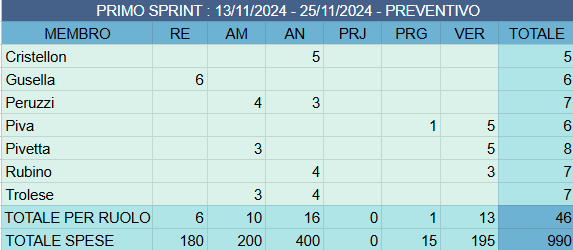
\includegraphics[width=0.6\linewidth]{preventivoOrePrimoSprint.png}
    	\caption{Preventivo orario per membro - Primo sprint}
    	\label{fig:Preventivo orario per membro - primo sprint}
    \end{figure}

    \begin{figure}[H]
        \centering
        \begin{tikzpicture}
            \pie[
                text=pin,
                hide number,
                color={responsabile, amministratore, analista, verificatore, programmatore}, 
                radius=1.5
            ]{13/Responsabile - 13\%, 22/Amministratore - 22\%, 35/Analista - 35\%, 28/Verificatore - 28\%, 2/Programmatore - 2\%}
        \end{tikzpicture}
        \caption{Diagramma circolare della partizione delle ore preventive per ruolo - Primo sprint }
        \label{fig:Diagramma circolare della partizione delle ore preventive per ruolo - primo sprint}
    \end{figure}
    
    \paragraph{Consuntivo orario}\mbox{}\vspace{0.4em}

    \begin{figure}[ht]
    	\centering
    	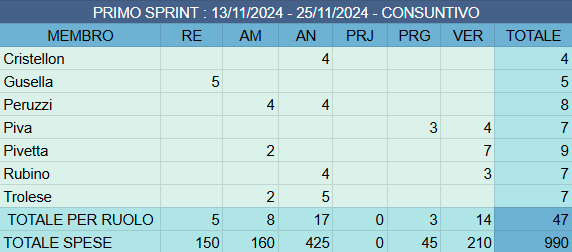
\includegraphics[width=0.6\linewidth]{consuntivoOrePrimoSprint.png}
    	\caption{Consuntivo orario per membro - Primo sprint}
    	\label{fig:Consuntivo orario per membro - primo sprint}
    \end{figure}

    \begin{figure}[H]
        \centering
        \begin{tikzpicture}
            \pie[
                text=pin,
                hide number,
                color={responsabile, amministratore, analista, verificatore, programmatore}, 
                radius=1.5
            ]{11/Responsabile - 11\%, 17/Amministratore - 17\%, 36/Analista - 36\%, 30/Verificatore - 30\%, 6/Programmatore - 6\%}
        \end{tikzpicture}
        \caption{Diagramma circolare della partizione delle ore consuntive per ruolo - Primo sprint }
        \label{fig:Diagramma circolare della partizione delle ore consuntive per ruolo - primo sprint}
    \end{figure}



    \paragraph{Rendicontazione delle risorse economiche restanti}\mbox{}\vspace{0.4em}

    
    \begin{figure}[ht]
    	\centering
    	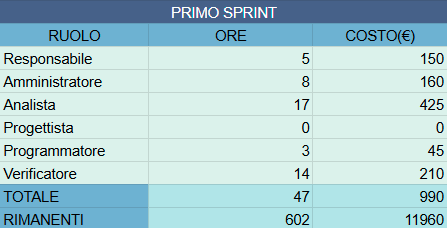
\includegraphics[width=0.6\linewidth]{oreCostiPrimoSprint.png}
    	\caption{Consuntivo orario e costi per ruolo - primo sprint}
    	\label{fig:Consuntivo orario e costi per ruolo - primo sprint}
    \end{figure}


    \paragraph{Retrospettiva}\mbox{}\vspace{0.4em}

    Durante il primo periodo di lavoro, CI$_G$ si è accorti quanto è fondamentale avere un way-of-working$_G$ ben definito, da seguire per l'intero progetto$_G$. Inoltre si è preso atto della difficoltà nel scrivere documentazione$_G$ esterna di qualità, seguendo normative, pertanto è probabile che i documenti subiscano numerose modifiche che riguardano stile e gergo.\\ Lo studio delle tecnologie richiede un ammontare di ore (non produttive) leggermente superiore a quanto previsto, pertanto è necessario chiarire i dubbi all'inizio per procedere successivamente in maniera lineare con l'implementazione delle varie librerie.\\Le task sono state distribuite in maniera abbastanza corretta, le attività sono state comunque terminate entro il tempo limite, sebbene a volte i verificatori hanno fatto notare qualche imprecisione nella qualità di documentazione$_G$.

%%%%%%%%%%
%%%%% Secondo sprint
%%%%%%%%%%%

\newpage
\subsubsection{Secondo sprint}
\label{secondo-sprint}
    
    \paragraph{Durata sprint}\mbox{}\\
    \vspace{-1.5em}
    \begin{table}[h] 
    \renewcommand{\arraystretch}{1.2}  
    \begin{tabular}{ l l }
        Inizio: & 2024-11-26 \\
        Fine Prevista: & 2024-12-05 \\
        Fine Effettiva: & 2024-12-05 \\
        Giorni di ritardo: & 0 \\
    \end{tabular}
    \end{table}
    \vspace{-2em}
    {\renewcommand{\arraystretch}{1.5}%
    
    \paragraph{Panoramica generale e obiettivi}\mbox{}\vspace{0.4em}
    
    Nel corso del secondo sprint$_G$ CI$_G$ si propone di avanzare con la redazione di tutta la documentazione$_G$, ma in particolare quella del documento di Analisi del Requisiti vista la richiesta della proponente$_G$ di visionarlo per valutarne la correttezza fino a questo punto. Sarà necessario anche procedere con la stesura delle sezioni mancanti nel documento Norme$_G$ di Progetto$_G$. Infine, dato che la durata dello sprint$_G$ sarà ridotta da due settimane a poco più di una a causa di motivi interni dell'azienda, occorrerà ridistribuire un buon ammontare di ore sulla parte che riguarda lo sviluppo del PoC$_G$, al fine di poterne presentare un prototipo con le funzioni più basiche accordate durante l'ultimo SAL$_G$.\\
    Seguono le attività nel backlog per questo periodo:
    \vspace{-0.5em}
    \begin{itemize}
    \setlength\itemsep{-0.2em}
    \item [-] Creazione di moduli software in seguito allo studio delle tecnologie approvate dalla proponente$_G$;
    \item [-] Migliorare l'ambiente di sviluppo docker-compose$_G$; 
    \item [-] Definire in dettaglio l'interazione con il framework$_G$ LLM$_G$;
    \item [-] Consuntivo primo sprint$_G$ nel Piano di Progetto$_G$;
    \item [-] Aggiunta use cases all'Analisi dei Requisiti;
    \item [-] Continuazione redazione delle Norme$_G$ di Progetto$_G$;
    \item [-] Integrazione di nuovi termini nel Glossario.
    \end{itemize}

    \paragraph{Gestione Rischi}\mbox{}
    \vspace{-1em}
    \subparagraph*{Rischi Attesi}\mbox{}
    
    Essendo nella fase più iniziale del progetto$_G$, i rischi in cui si aspetta di imbattersi sono vari. Fra tutti, sono stati selezionati:
    \vspace{-0.5em}
    \begin{itemize}
    \setlength\itemsep{-0.2em}
    \item [-] \hyperref[RT1]{RT1} - Complessità delle nuove tecnologie;
    \item [-] \hyperref[RT2]{RT2} - Carenza di documentazione$_G$ sulle tecnologie;
    \item [-] \hyperref[RT3]{RT3} - Produzione di codice confuso o con errori;
    \item [-] \hyperref[RC3]{RC3} - Cambio dei ruoli;
    \item [-] \hyperref[RP1]{RP1} - Impegni al di fuori del progetto$_G$ o indisponibilità individuale
    \end{itemize}

    \subparagraph*{Rischi Incontrati}\mbox{}
    
    Durante il secondo periodo il gruppo si è scontrato in particolare con il rischio$_G$ dell'indisponibilità individuale \hyperref[RP1]{RP1}. Come era stato comunicato durante il primo SAL$_G$, il tempo di questo sprint$_G$ è stato dimezzato a causa dell'indisponibilità del responsabile della proponente$_G$. Questo ha comportato un investimento del monte ore molto maggiore rispetto ad una normale settimana di sprint$_G$, al fine di produrre qualcosa di significativamente presentabile durante il successivo SAL$_G$. Inoltre durante la settimana un membro del team, a causa di motivi di salute, è stato impossibilitato a lavorare, e questo spiega il basso numero di ore produttive. Questo rischio$_G$ è stato mitigato grazie ad altri membri del team che si sono occupati di ricoprire le task pendenti. Come nel primo sprint$_G$, CI$_G$ si è imbattuti in problemi con la documentazione$_G$ di alcune tecnologie che risultava poco chiara (\hyperref[RT2]{RT2}). Questi sono stati limitati grazie ad una sessione di peer programming che ha permesso di individuare ed eliminare alcuni bug$_G$ nel PoC$_G$. Infine, a causa del cambio dei ruoli (\hyperref[RC3]{RC3}), i nuovi analisti di questo sprint$_G$ hanno avuto dei dubbi in ambito di redazione degli use cases, risolti in aula grazie a delle delucidazioni del docente. 

    
    \paragraph{Definizione ruoli}\mbox{}\vspace{0.4em}
    
    Questi sono i ruoli assegnati per membro in questo secondo sprint$_G$.\\
    \begin{table}[H]
        \centering
        \begin{tabular}{|c|c|}
        \hline
        \rowcolor{gray!25}
        \textbf{Ruolo} & \textbf{Membro}\\
        \hline
        Responsabile & Uncas Peruzzi\\
        \hline
        Amministratore & Alfredo Rubino\\ 
        \hline
        Analista & Federico Pivetta\\
        & Manuel Gusella \\
        & Riccardo Piva\\
        \hline
        Progettista & / \\
        \hline
        Programmatore & / \\
        \hline
        Verificatore & Giovanni Cristellon\\
        & Leonardo Trolese\\
        \hline
        \end{tabular}
        \caption{Tabella dei ruoli - Secondo Sprint}
        %\label{tab:my_label}
    \end{table}

    \paragraph{Preventivo orario}\mbox{}\vspace{0.4em}
    \begin{figure}[ht]
    	\centering
    	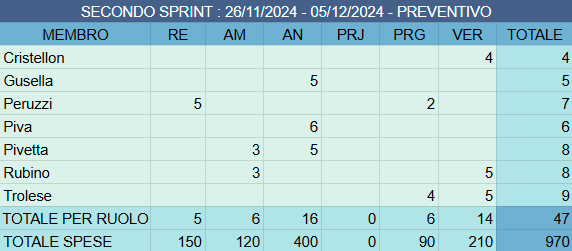
\includegraphics[width=0.6\linewidth]{preventivoOreSecondoSprint.png}
    	\caption{Preventivo orario per membro - Secondo sprint}
    	\label{fig:Preventivo orario per membro - Secondo sprint}
    \end{figure}

    \begin{figure}[H]
        \centering
        \begin{tikzpicture}
            \pie[
                text=pin,
                hide number,
                color={responsabile, amministratore, analista, verificatore, programmatore}, 
                radius=1.5
            ]{11/Responsabile - 11\%, 16/Amministratore - 16\%, 34/Analista - 34\%, 30/Verificatore - 30\%, 9/Programmatore - 9\%}
        \end{tikzpicture}
        \caption{Diagramma circolare della partizione delle ore preventive per ruolo - Secondo sprint }
        \label{fig:Diagramma circolare della partizione delle ore preventive per ruolo - Secondo sprint}
    \end{figure}
    
    \paragraph{Consuntivo orario}\mbox{}\vspace{0.4em}
    \begin{figure}[ht]
    	\centering
    	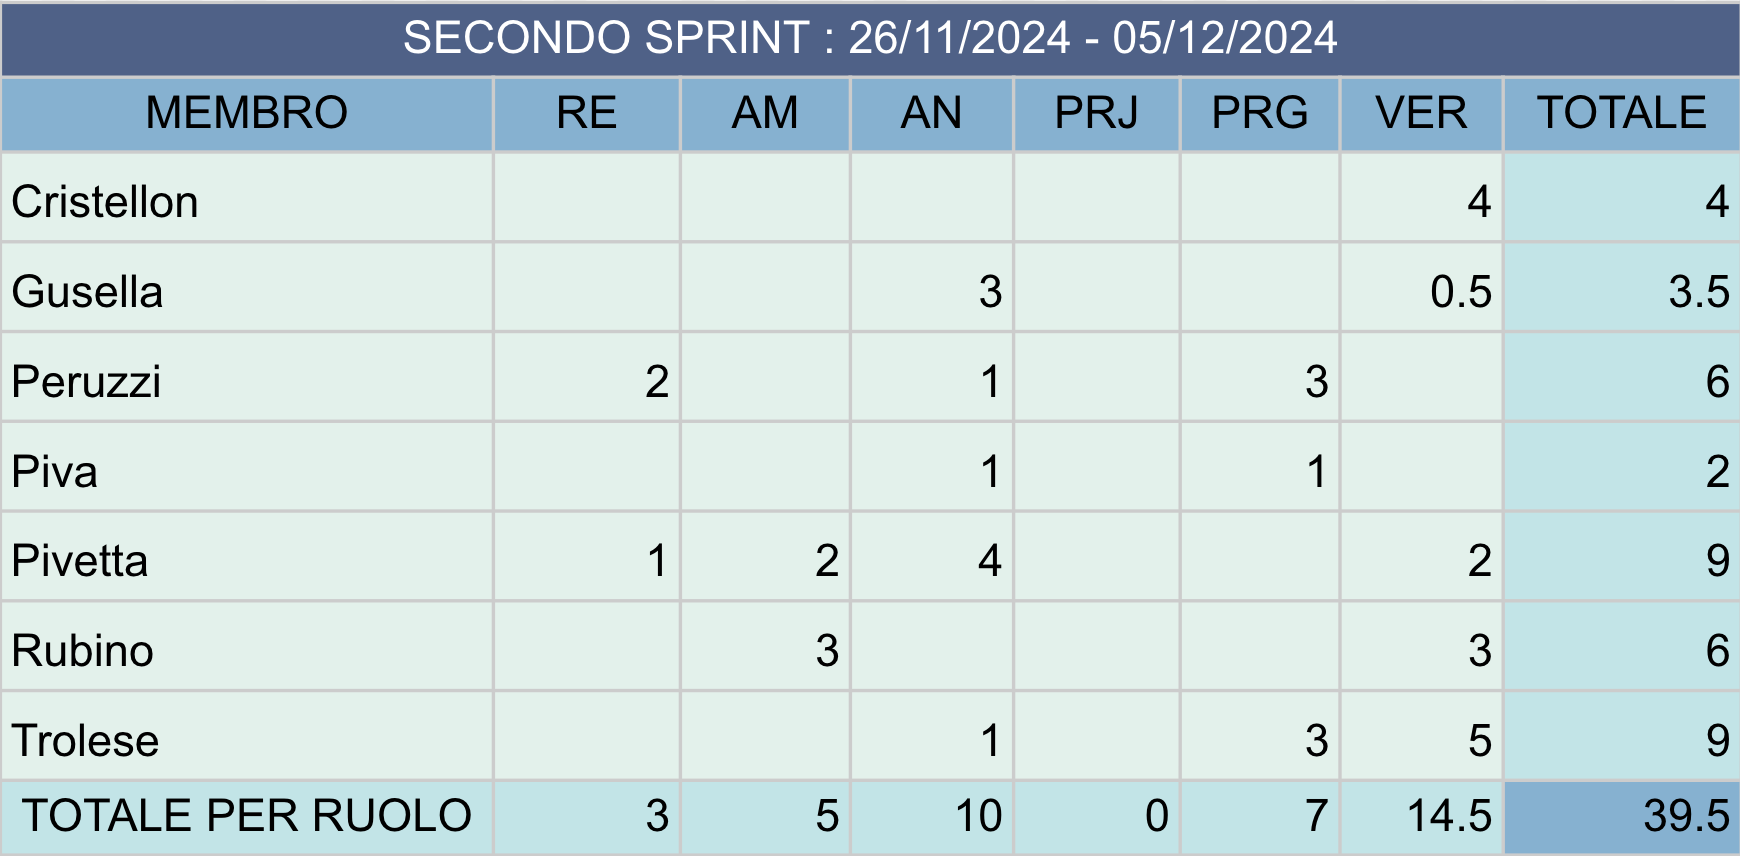
\includegraphics[width=0.6\linewidth]{consuntivoOreSecondoSprint.png}
    	\caption{Consuntivo orario per membro - Secondo sprint}
    	\label{fig:Consuntivo orario per membro - secondo sprint}
    \end{figure}

    \begin{figure}[H]
        \centering
        \begin{tikzpicture}
            \pie[
                text=pin,
                hide number,
                color={responsabile, amministratore, analista, programmatore, verificatore}, 
                radius=1.5
            ]{13/Responsabile - 13\%, 11/Amministratore - 11\%, 31/Analista - 31\%, 18/Programmatore - 18\%, 27/Verificatore - 27\%}
        \end{tikzpicture}
        \caption{Diagramma circolare della partizione delle ore consuntive per ruolo - Secondo sprint }
        \label{fig:Diagramma circolare della partizione delle ore consuntive per ruolo - secondo sprint}
    \end{figure}

    \paragraph{Rendicontazione delle risorse economiche restanti}\mbox{}\vspace{0.4em}
    \begin{figure}[H]
    	\centering
    	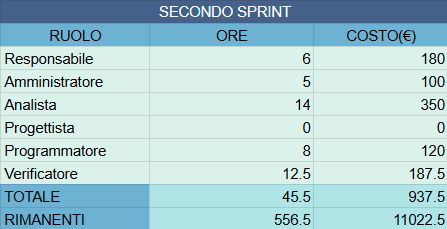
\includegraphics[width=0.6\linewidth]{oreCostiSecondoSprint.png}
    	\caption{Consuntivo orario e costi per ruolo - Secondo sprint}
    	\label{fig:Consuntivo orario e costi per ruolo - Secondo sprint}
    \end{figure}
    
    \paragraph{Retrospettiva}\mbox{}\vspace{0.4em}
    
    Il secondo sprint$_G$ è stato molto importante, in quanto ha permesso al team di capire come essere il più produttivi possibile in tempi ristretti a causa di indisponibilità di uno o più membri. Oltre a ciò, si è visto anche quanto la comunicazione sia importante tra i membri del team, in caso di ridistribuzione di task varie.\\ 
    \'E stato sicuramente notato quanto sia comodo ed efficiente avere un ambiente di sviluppo e di deployment solido e privo di bug$_G$.\\ 
    \'E stato inoltre rilevato un buon approccio da parte dei verificatori, che hanno rilevato errori e imprecisioni in alcuni documenti permettendo la modifica tempestiva.\\ 
    Il secondo SAL$_G$ è servito per garantirci la corretta e solida base del documento di Analisi-dei-requisiti$_G$ e l'approvazione del prototipo del PoC$_G$, con alcuni miglioramenti in termini di prestazione e performance del software.\\ 
    L'incontro intermedio con l'azienda, sebbene di breve durata, è risultato utile per chiarire alcune incertezze, mentre il SAL$_G$ ha permesso di capire in che modo vanno presentati i progressi conseguiti, in modo da permettere alla proponente$_G$ di essere sincronizzata sul programma del team.
    
%%%%%%%%%%
%%%%% Terzo sprint
%%%%%%%%%%%

\newpage
\subsubsection{Terzo sprint}
\label{terzo-sprint}
    
    \paragraph{Durata sprint}\mbox{}\\
    \vspace{-1.5em}
    \begin{table}[h] 
    \renewcommand{\arraystretch}{1.2}  
    \begin{tabular}{ l l }
        Inizio: & 2024-12-06 \\
        Fine Prevista: & 2024-12-20 \\
        Fine Effettiva: & 2024-12-20 \\
        Giorni di ritardo: & 0 \\
    \end{tabular}
    \end{table}
    \vspace{-2em}
    {\renewcommand{\arraystretch}{1.5}%
    
    \paragraph{Panoramica generale e obiettivi}\mbox{}\vspace{0.4em}

    Nel corso del terzo sprint$_G$, il gruppo si propone di proseguire la redazione e il perfezionamento della documentazione$_G$ prodotta fino a questo momento, avviare la stesura del documento \textit{Piano\_di\_Qualifica.pdf} e approfondire ulteriormente il prototipo del PoC$_G$ presentato alla proponente$_G$ durante lo sprint$_G$ precedente. Questo approfondimento include l'implementazione delle chiavi Kafka$_G$, la generazione di un numero consistente di punti di interesse, il miglioramento del messaggio generato dalla LLM$_G$ e l'integrazione delle due parti del PoC$_G$ precedentemente sviluppate in un unico modulo. Inoltre, prima dell'inizio del quarto sprint$_G$, è stato deciso di organizzare un incontro con il committente$_G$, Professor Cardin, al fine di chiarire alcuni dubbi sugli use case.\\
    Seguono le attività nel backlog per questo periodo:
    \vspace{-0.5em}
    \begin{itemize}
    \setlength\itemsep{-0.2em}
    \item [-] Studio e implementazioni chiavi Kafka$_G$;
    \item [-] Approfondimento del messaggio generato dall'LLM;
    \item [-] Studio e generazione dei punti di interesse sulla dashboard$_G$;
    \item [-] Consuntivo secondo sprint$_G$ nel Piano di Progetto$_G$;
    \item [-] Continuazione redazione delle Norme$_G$ di Progetto$_G$;
    \item [-] Inizio stesura Piano di Qualifica;
    \item [-] Integrazione di nuovi termini nel Glossario.
    \end{itemize}

    \paragraph{Gestione Rischi}\mbox{}
    \vspace{-1em}
    \subparagraph*{Rischi Attesi}\mbox{}
    Essendo iniziata la fase intermedia del progetto$_G$, i rischi in cui si aspetta di imbattersi sono vari. Fra tutti, sono stati selezionati:
    \vspace{-0.5em}
    \begin{itemize}
    \setlength\itemsep{-0.2em}
    \item [-] \hyperref[RT1]{RT1} - Complessità delle nuove tecnologie;
    \item [-] \hyperref[RT3]{RT3} - Produzione di codice confuso o con errori;
    \item [-] \hyperref[RP2]{RP2} - Incertezza sulla stime delle attività.
    \end{itemize}

    \subparagraph*{Rischi Incontrati}\mbox{}

    Durante il terzo periodo, il gruppo ha affrontato i rischi precedentemente identificati. Analogamente agli sprint$_G$ passati, sono emerse difficoltà nell'utilizzo di alcune tecnologie (\hyperref[RT1]{RT1}) necessarie per affrontare le criticità e migliorare gli aspetti evidenziati nel SAL$_G$ precedente. Nel tentativo di individuare la soluzione più idonea per soddisfare le ultime richieste relative al PoC$_G$, è stato prodotto un codice inizialmente confuso (\hyperref[RT3]{RT3}). Tuttavia, grazie a una comunicazione attiva e chiara tra i membri del gruppo, è stato possibile risolvere questo problema.
    Infine, durante la stesura asincrona di nuove sezioni della documentazione$_G$, soprattutto a causa della loro natura complessa, sono emerse difficoltà legate alla stima delle attività (\hyperref[RP2]{RP2}). Tali difficoltà sono state successivamente risolte mediante un utilizzo sistematico ed esaustivo delle issue$_G$, che ha consentito un'organizzazione e una gestione delle task più efficiente.
    
    \paragraph{Definizione ruoli}\mbox{}\vspace{0.4em}
    
    Questi sono i ruoli assegnati per membro in questo terzo sprint$_G$.\\
    \begin{table}[H]
        \centering
        \begin{tabular}{|c|c|}
        \hline
        \rowcolor{gray!25}
        \textbf{Ruolo} & \textbf{Membro}\\
        \hline
        Responsabile & Federico Pivetta\\
        \hline
        Amministratore & Leonardo Trolese\\ 
        \hline
        Analista & Uncas Peruzzi\\
        & Riccardo Piva\\
        \hline
        Progettista & / \\
        \hline
        Programmatore & Giovanni Cristellon \\
        \hline
        Verificatore & Manuel Gusella\\
        & Alfredo Rubino\\
        \hline
        \end{tabular}
        \caption{Tabella dei ruoli - Terzo Sprint}
        %\label{tab:my_label}
    \end{table}

    \paragraph{Preventivo orario}\mbox{}\vspace{0.4em}
    \begin{figure}[H]
    	\centering
    	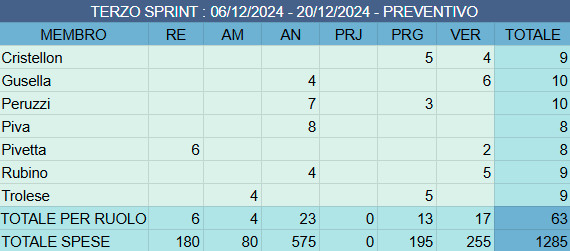
\includegraphics[width=0.6\linewidth]{preventivoOreTerzoSprint.PNG}
    	\caption{Preventivo orario per membro - Terzo sprint}
    	\label{fig:Preventivo orario per membro - Terzo sprint}
    \end{figure}

    \begin{figure}[H]
        \centering
        \begin{tikzpicture}
            \pie[
                text=pin,
                hide number,
                color={responsabile, amministratore, analista, programmatore, verificatore}, 
                radius=1.5
            ]{10/Responsabile - 10\%, 6/Amministratore - 6\%, 37/Analista - 37\%, 21/Programmatore - 21\%, 27/Verificatore - 27\%}
        \end{tikzpicture}
        \caption{Diagramma circolare della partizione delle ore preventive per ruolo - Terzo sprint }
        \label{fig:Diagramma circolare della partizione delle ore preventive per ruolo - Terzo sprint}
    \end{figure}
    
    \paragraph{Consuntivo orario}\mbox{}\vspace{0.4em}
    \begin{figure}[ht]
    	\centering
    	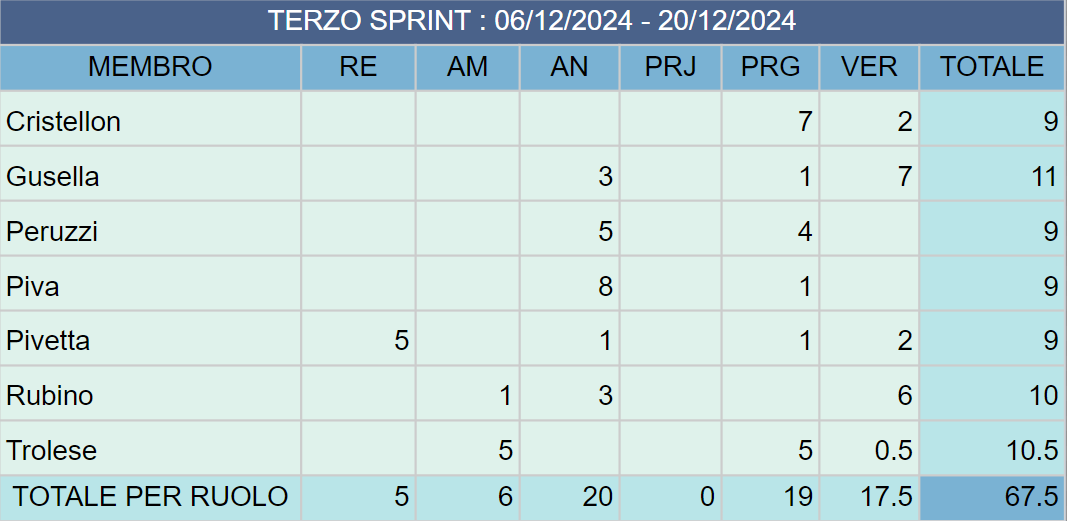
\includegraphics[width=0.6\linewidth]{consuntivoOreTerzoSprint.PNG}
    	\caption{Consuntivo orario per membro - Terzo sprint}
    	\label{fig:Consuntivo orario per membro - terzo sprint}
    \end{figure}

    \begin{figure}[H]
        \centering
        \begin{tikzpicture}
            \pie[
                text=pin,
                hide number,
                color={responsabile, amministratore, analista, programmatore, verificatore}, 
                radius=1.5
            ]{8/Responsabile - 8\%, 9/Amministratore - 9\%, 31/Analista - 31\% , 25/Programmatore - 25\%, 27/Verificatore - 27\%}
        \end{tikzpicture}
        \caption{Diagramma circolare della partizione delle ore consuntive per ruolo - Terzo sprint }
        \label{fig:Diagramma circolare della partizione delle ore consuntive per ruolo - terzo sprint}
    \end{figure}

    \paragraph{Rendicontazione delle risorse economiche restanti}\mbox{}\vspace{0.4em}
    \begin{figure}[H]
    	\centering
    	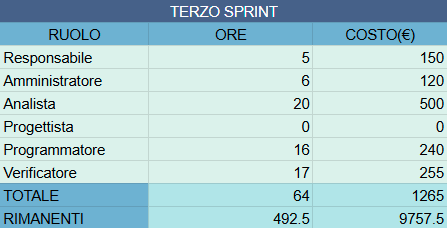
\includegraphics[width=0.6\linewidth]{oreCostiTerzoSprint.PNG}
    	\caption{Consuntivo orario e costi per ruolo - Terzo sprint}
    	\label{fig:Consuntivo orario e costi per ruolo - Terzo sprint}
    \end{figure}
    
    \paragraph{Retrospettiva}\mbox{}\vspace{0.4em}

    Il terzo sprint$_G$ ha consentito al gruppo di acquisire una maggiore familiarità con le nuove tecnologie, analizzandone sia i vantaggi che gli svantaggi associati a ciascuna di esse.\\
    Il processo$_G$ di verifica è stato ulteriormente perfezionato, garantendo una segnalazione più immediata delle eventuali correzioni da apportare direttamente tramite GitHub$_G$.\\
    L'incontro intermedio con la proponente$_G$ si è rivelato utile per chiarire alcune incertezze, mentre il terzo SAL$_G$ ha fornito un feedback$_G$ sul prototipo del PoC$_G$ sviluppato fino a quel momento, evidenziando i punti su cui concentrare il lavoro una volta superata la revisione RTB$_G$.\\
    Il ricevimento con il professor Riccardo Cardin è stato determinante per comprendere come redigere un documento di analisi-dei-requisiti$_G$ nel modo più corretto possibile e in grado di apportare un valore aggiunto al progetto$_G$; inoltre, ha permesso di risolvere un dubbio relativo agli attori nei casi d'uso.\\
    Questo sprint$_G$ ha ulteriormente evidenziato l'importanza di una documentazione$_G$ accurata e di un'organizzazione consolidata, indispensabili per garantire lo svolgimento efficace ed efficiente di un progetto$_G$ collaborativo.

%%%%%%%%%%
%%%%% Quarto sprint
%%%%%%%%%%%

\newpage
\subsubsection{Quarto sprint}
\label{quarto-sprint}
    
    \paragraph{Durata sprint}\mbox{}\\
    \vspace{-1.5em}
    \begin{table}[h] 
    \renewcommand{\arraystretch}{1.2}  
    \begin{tabular}{ l l }
        Inizio: & 2024-12-21 \\
        Fine Prevista: & 2025-01-08 \\
        Fine Effettiva: & 2025-01-08 \\
        Giorni di ritardo: & 0 \\
    \end{tabular}
    \end{table}
    \vspace{-2em}
    {\renewcommand{\arraystretch}{1.5}%
    
    \paragraph{Panoramica generale e obiettivi}\mbox{}\vspace{0.4em}

    Nel corso del quarto sprint$_G$ il team prevede di continuare la stesura della documentazione$_G$ e la produzione del PoC$_G$. Nello specifico 
    il gruppo si concentrerà proprio sulla documentazione$_G$ con particolare interesse alla modifica e al perfezionamento del documento di
    Analisi-dei-requisiti$_G$, a seguito del confronto avvenuto in data 2024-12-20 con il professor Cardin. Il gruppo si propone nel corso di
    questa iterazione di terminare la redazione di tutti i documenti in vista della consegna RTB$_G$ prevista che il gruppo prevede di
    effettuare entro la prima metà di gennaio 2025. Sebbene presente si prevede meno tempo produttivo da destinare al PoC$_G$ poiché a seguito
    di un confronto con al proponente$_G$ quanto fatto fino ad ora è stato ritenuto sufficiente a provare la fattibilità del progetto$_G$.\\
    Seguono le attività inserite nel backlog per questo periodo:
    \vspace{-0.5em}
    \begin{itemize}
    \setlength\itemsep{-0.2em}
    \item [-] Correzione dell'Analisi dei Requisiti a seguito delle indicazioni del professor Cardin;
    \item [-] Aggiunta di ulteriori UC all'Analisi dei Requisiti;
    \item [-] Redazione della sezione relativa alle metriche nelle Norme$_G$ di Progetto$_G$;
    \item [-] Correzione della sezione relativa agli standard nelle Norme$_G$ di Progetto$_G$;
    \item [-] Redazione delle sezioni di gestione della configurazione, miglioramento e formazione nelle Norme$_G$ di Progetto$_G$;
    \item [-] Calcolo e rendicontazione delle metriche utili per la consegna RTB$_G$ relativamente ai primi tre sprint$_G$;
    \item [-] Correzione dell'implementazione dei topic$_G$ Kafka$_G$ nel PoC$_G$;
    \item [-] Consuntivo terzo sprint$_G$ nel Piano di Progetto$_G$;
    \item [-] Inizio stesura Piano di Qualifica;
    \item [-] Integrazione di nuovi termini nel Glossario.
    \end{itemize}

    \paragraph{Gestione Rischi}\mbox{}
    \vspace{-1em}
    \subparagraph*{Rischi Attesi}\mbox{}
    Relativamente alla quarta iterazione sono stati identificati dei potenziali rischi in cui potrebbe imbattersi il gruppo:
    \vspace{-0.5em}
    \begin{itemize}
    \setlength\itemsep{-0.2em}
    \item [-] \hyperref[RT1]{RT1} - Complessità delle nuove tecnologie;
    \item [-] \hyperref[RC1]{RC1} - Comunicazione interna non ottimale;
    \item [-] \hyperref[RC3]{RC3} - Cambio dei ruoli;
    \end{itemize}

    \subparagraph*{Rischi Incontrati}\mbox{}

    Nel corso del quarto periodo il gruppo ha riscontrato e affrontato positivamente una parte dei rischi previsti per questa iterazione.
    Poiché questo sprint$_G$ si è sovrapposto al periodo festivo e natalizio, erano stati previsti dei problemi di comunicazione e coordinazione
    tra i membri del gruppo dovuti ai numerosi impegni individuali. Il rischio$_G$ si è rivelato fondato, e in diverse occasioni
    la coordinazione del gruppo ne ha risentito (\hyperref[RC1]{RC1}), tanto che durante un incontro intermedio informale dei membri 
    meno della metà ha presenziato.\\
    Anche le tecnologie si sono rivelate problematiche poiché sono sorte delle difficoltà nella gestione dei topic$_G$ Kafka$_G$ (\hyperref[RT1]{RT1}), 
    prontamente risolte all'inizio dello sprint$_G$.\\
    Il rischio$_G$ inizialmente previsto per il cambio dei ruoli (\hyperref[RC3]{RC3}) si è invece rivelato infondato poiché il gruppo non ne ha risentito.
    
    \paragraph{Definizione ruoli}\mbox{}\vspace{0.4em}
    
    Questi sono i ruoli assegnati per membro in questo quarto sprint$_G$.\\
    \begin{table}[H]
        \centering
        \begin{tabular}{|c|c|}
        \hline
        \rowcolor{gray!25}
        \textbf{Ruolo} & \textbf{Membro}\\
        \hline
        Responsabile & Leonardo Trolese\\
        \hline
        Amministratore & Federico Pivetta\\ 
        \hline
        Analista & Manuel Gusella\\
        & Giovanni Cristellon\\
        & Alfredo Rubino\\
        \hline
        Progettista & / \\
        \hline
        Programmatore & Uncas Peruzzi \\
        \hline
        Verificatore & Riccardo Piva\\
        \hline
        \end{tabular}
        \caption{Tabella dei ruoli - Quarto Sprint}
        %\label{tab:my_label}
    \end{table}

    \paragraph{Preventivo orario}\mbox{}\vspace{0.4em}
    \begin{figure}[H]
    	\centering
    	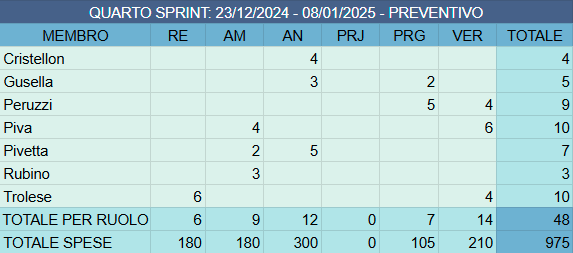
\includegraphics[width=0.6\linewidth]{preventivoOreQuartoSprint.PNG}
    	\caption{Preventivo orario per membro - Quarto sprint}
    	\label{fig:Preventivo orario per membro - Quarto sprint}
    \end{figure}

    \begin{figure}[H]
        \centering
        \begin{tikzpicture}
            \pie[
                text=pin,
                hide number,
                color={responsabile, amministratore, analista, programmatore, verificatore}, 
                radius=1.5
            ]{12/Responsabile - 12\%, 19/Amministratore - 19\%, 25/Analista - 25\% , 15/Programmatore - 15\%, 29/Verificatore - 29\%}
        \end{tikzpicture}
        \caption{Diagramma circolare della partizione delle ore preventive per ruolo - Quarto sprint }
        \label{fig:Diagramma circolare della partizione delle ore preventive per ruolo - Quarto sprint}
    \end{figure}
    
    \paragraph{Consuntivo orario}\mbox{}\vspace{0.4em}
    \begin{figure}[ht]
    	\centering
    	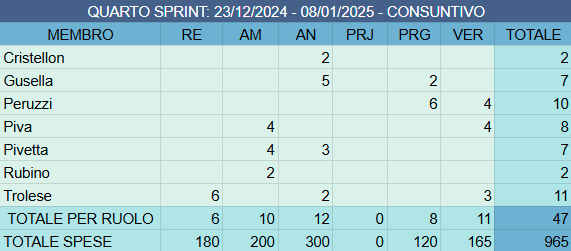
\includegraphics[width=0.6\linewidth]{consuntivoOreQuartoSprint.PNG}
    	\caption{Consuntivo orario per membro - Quarto sprint}
    	\label{fig:Consuntivo orario per membro - quarto sprint}
    \end{figure}

    \begin{figure}[H]
        \centering
        \begin{tikzpicture}
            \pie[
                text=pin,
                hide number,
                color={responsabile, amministratore, analista, programmatore, verificatore}, 
                radius=1.5
            ]{13/Responsabile - 13\%, 20/Amministratore - 20\%, 26/Analista - 26\% , 17/Programmatore - 17\%, 24/Verificatore - 24\%}
        \end{tikzpicture}
        \caption{Diagramma circolare della partizione delle ore consuntive per ruolo - Quarto sprint }
        \label{fig:Diagramma circolare della partizione delle ore consuntive per ruolo - quarto sprint}
    \end{figure}

    \paragraph{Rendicontazione delle risorse economiche restanti}\mbox{}\vspace{0.4em}
    \begin{figure}[H]
    	\centering
    	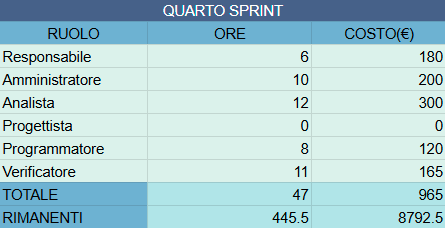
\includegraphics[width=0.6\linewidth]{oreCostiQuartoSprint.PNG}
    	\caption{Consuntivo orario e costi per ruolo - Quarto sprint}
    	\label{fig:Consuntivo orario e costi per ruolo - Quarto sprint}
    \end{figure}
    
    \paragraph{Retrospettiva}\mbox{}\vspace{0.4em}

    Il quarto sprint$_G$ ha centrato l'attenzione del gruppo sulla redazione della documentazione$_G$ allo scopo di ultimare la stesura dei 
    documenti utili alla consegna RTB$_G$: è stata completata l'Analisi dei Requisiti, e sono state quasi ultimate anche le Norme$_G$ di Progetto$_G$.\\
    Durante la retrospettiva i membri hanno esposto il lavoro svolto durante la quarta iterazione, ed è emersa una costruttiva discussione
    sulle metriche adottate, sulla loro implementazione e sulla loro presentazione all'interno del Piano di Qualifica.\\
    L'obiettivo del quarto sprint$_G$ consisteva nella terminazione della redazione di tutta la documentazione$_G$, e sebbene tutti i documenti siano
    stati in gran parte completati, l'obiettivo non è stato pienamente raggiunto; si è pertanto deciso di concludere la stesura dei documenti,
    insieme alla loro verifica conclusiva, nel corso del periodo a venire.


%%%%%%%%%%
%%%%% Quinto sprint
%%%%%%%%%%%

\newpage
\subsubsection{Quinto sprint}
\label{quinto-sprint}
    
    \paragraph{Durata sprint}\mbox{}\\
    \vspace{-1.5em}
    \begin{table}[h] 
    \renewcommand{\arraystretch}{1.2}  
    \begin{tabular}{ l l }
        Inizio: & 2025-01-09 \\
        Fine Prevista: & 2025-01-24 \\
        Fine Effettiva: & 2025-01-29 \\
        Giorni di ritardo: & 5 \\
    \end{tabular}
    \end{table}
    \vspace{-2em}
    {\renewcommand{\arraystretch}{1.5}%
    
    \paragraph{Panoramica generale e obiettivi}\mbox{}\vspace{0.4em}

Nel corso del quinto sprint$_G$ il gruppo si propone di continuare e ultimare la redazione della documentazione$_G$ per la consegna RTB$_G$.
    In particolare si prevede di concentrarsi su documenti come il Piano di Qualifica e l'Analisi dei Requisiti.\\
    Inoltre il gruppo:
    \begin{itemize}
        \item Programmerà un incontro con il professor Cardin per discutere del lavoro svolto e per ricevere eventuali feedback$_G$;
        \item Invierà i documenti all'azienda per ricevere una revisione.
    \end{itemize}
    Le attività previste sono poche e molto concentrate; inoltre, questo sprint$_G$ potrebbe risentire del periodo degli esami universitari.\\

    Seguono le attività inserite nel backlog per questo periodo:
    \vspace{-0.5em}
    \begin{itemize}
    \setlength\itemsep{-0.2em}
    \item [-] Aggiunta di ulteriori UC al documento di Analisi-dei-requisiti$_G$ in seguito al primo ricevimento con il professor Cardin;
    \item [-] Analisi tecnologie per contrastare il kafka$_G$ poisoning;
    \item [-] Correzione del documento di analisi-dei-requisiti$_G$ a seguito delle indicazioni ricevuti nel secondo ricevimento con il professor Cardin;
    \item [-] Redazione sezione test$_G$ di sistema$_G$, test$_G$ d'integrazione e test$_G$ di accettazione nel Piano di Qualifica;
    \item [-] Redazione cruscotto$_G$ nel Piano di Qualifica;
    \item [-] Calcolo e generazione dei grafici da inserire nel cruscotto$_G$ del Piano di Qualifica;
    \item [-] Consuntivo quarto sprint$_G$ nel Piano di Progetto$_G$;
    \item [-] Integrazione di nuovi termini nel Glossario.
    \end{itemize}

    \paragraph{Gestione Rischi}\mbox{}
    \vspace{-1em}
    \subparagraph*{Rischi Attesi}\mbox{}
    
    Relativamente alla quinta iterazione sono stati identificati dei potenziali rischi in cui potrebbe imbattersi il gruppo:
    \vspace{-0.5em}
    \begin{itemize}
    \setlength\itemsep{-0.2em}
    \item [-] \hyperref[RP2]{RP2} - Incertezza sulle stime delle attività;
    \item [-] \hyperref[RP1]{RP1} - Impegni al di fuori del progetto$_G$ o indisponibilità individuale;
    \item [-] \hyperref[RC3]{RC3} - Cambio dei ruoli;
    \item [-] \hyperref[RP3]{RP3} - Rischio$_G$ cambiamenti improvvisi a ridosso della consegna;
    \end{itemize}

    \subparagraph*{Rischi Incontrati}\mbox{}

    Nel corso del quinto periodo il gruppo ha riscontrato e affrontato positivamente una parte dei rischi previsti per questa iterazione.
    Questo sprint$_G$ è avvenuto durante il periodo degli esami universitari e questo ha comportato un rallentamento nella redazione della documentazione$_G$.
    Di conseguenza il gruppo, data la riduzione di produttività ha deciso di allungare lo sprint$_G$ di qualche giorno e posticipare la consegna RTB$_G$ alla prossima iterazione.

    \paragraph{Definizione ruoli}\mbox{}\vspace{0.4em}
    
    Questi sono i ruoli assegnati per membro in questo quinto sprint$_G$.\\
    \begin{table}[H]
        \centering
        \begin{tabular}{|c|c|}
        \hline
        \rowcolor{gray!25}
        \textbf{Ruolo} & \textbf{Membro}\\
        \hline
        Responsabile & Riccardo Piva\\
        \hline
        Amministratore & Manuel Gusella \\ 
        \hline
        Analista & Giovanni Cristellon \\
        & Federico Pivetta \\
        \hline
        Progettista & / \\
        \hline
        Programmatore & / \\
        \hline
        Verificatore & Leonardo Trolese \\
        & Alfredo Rubino \\
        & Uncas Peruzzi \\
        \hline
        \end{tabular}
        \caption{Tabella dei ruoli - Quinto Sprint}
    \end{table}

    \paragraph{Preventivo orario}\mbox{}\vspace{0.4em}
    \begin{figure}[H]
    	\centering
    	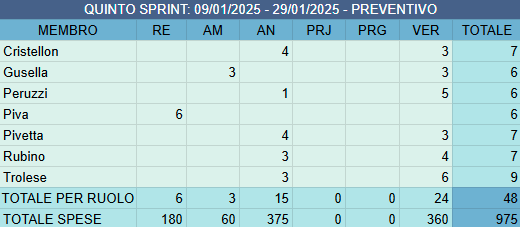
\includegraphics[width=0.6\linewidth]{preventivoOreQuintoSprint.PNG}
    	\caption{Preventivo orario per membro - Quinto sprint}
    	\label{fig:Preventivo orario per membro - Quinto sprint}
    \end{figure}

    \begin{figure}[H]
        \centering
        \begin{tikzpicture}
            \pie[
                text=pin,
                hide number,
                color={responsabile, amministratore, analista, verificatore}, 
                radius=1.5
            ]{13/Responsabile - 13\%, 6/Amministratore - 6\%, 31/Analista - 31\% , 50/Verificatore - 50\%}
        \end{tikzpicture}
        \caption{Diagramma circolare della partizione delle ore preventive per ruolo - Quinto sprint }
        \label{fig:Diagramma circolare della partizione delle ore preventive per ruolo - Quinto sprint}
    \end{figure}
    
    \paragraph{Consuntivo orario}\mbox{}\vspace{0.4em}
    \begin{figure}[ht]
    	\centering
    	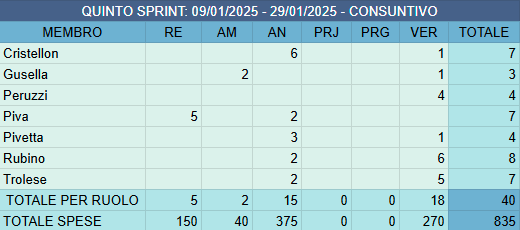
\includegraphics[width=0.6\linewidth]{consuntivoOreQuintoSprint.png}
    	\caption{Consuntivo orario per membro - Quinto sprint}
\label{fig:Consuntivo orario per membro - Quinto sprint}
    \end{figure}

    \begin{figure}[H]
        \centering
        \begin{tikzpicture}
            \pie[
                text=pin,
                hide number,
                color={responsabile, amministratore, analista, verificatore}, 
                radius=1.5
            ]{12/Responsabile - 12\%, 5/Amministratore - 5\%, 38/Analista - 38\% , 45/Verificatore - 45\%}
        \end{tikzpicture}
        \caption{Diagramma circolare della partizione delle ore consuntive per ruolo - Quinto sprint }
        \label{fig:Diagramma circolare della partizione delle ore consuntive per ruolo - Quinto sprint}
    \end{figure}

    \paragraph{Rendicontazione delle risorse economiche restanti}\mbox{}\vspace{0.4em}
    \begin{figure}[H]
    	\centering
    	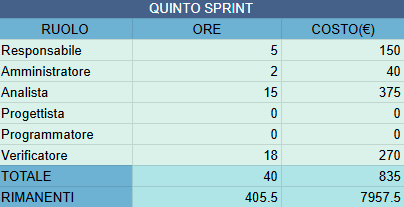
\includegraphics[width=0.6\linewidth]{oreCostiQuintoSprint.png}
    	\caption{Consuntivo orario e costi per ruolo - Quinto sprint}
    	\label{fig:Consuntivo orario e costi per ruolo - Quinto sprint}
    \end{figure}
    
    \paragraph{Retrospettiva}\mbox{}\vspace{0.4em}

    Il quinto sprint$_G$ ha evidenziato diverse difficoltà, principalmente legate alla conclusione dei documenti necessari per la consegna RTB$_G$. La fase di redazione è stata particolarmente impegnativa a causa dei numerosi cambiamenti richiesti.
    Durante la prima riunione con il professor Cardin erano emerse alcune criticità legate alla separazione dei sistemi all'interno dell'Analisi dei Requisiti, che hanno richiesto le creazione di alcuni UC per chiarire meglio il funzionamento del sistema$_G$. 
    Inoltre è emersa anche una potenziale vulnerabilità legata al kafka$_G$ poisoning, per cui c'è stato un confronto con l'azienda e di conseguenza un'analisi per trovare un'eventuale soluzione adeguata.
    Durante questo sprint$_G$ sono stati redatte numerose sezioni del Piano di Qualifica, tra cui la sezione dei test$_G$ e  il cruscotto$_G$, con conseguente calcolo delle metriche da inserire.
    Durante una seconda riunione con il professor Cardin, sono emerse ulteriori modifiche da apportare al documento di Analisi-dei-requisiti$_G$, il che ha reso necessario posticipare la consegna RTB$_G$. 
    La riunione è stata fondamentale per chiarire alcuni aspetti critici, ma ha anche comportato un ulteriore carico di lavoro per il team.
    In aggiunta, il periodo degli esami universitari ha significativamente ridotto la disponibilità dei membri del gruppo, rallentando il progresso complessivo. 
    Nonostante ciò, il team ha cercato di mantenere un ritmo costante, ma la pressione degli esami ha inevitabilmente influito sulla produttività.
    Infine, una riunione conclusiva con l'azienda ha permesso di fare il punto della situazione e di pianificare le attività rimanenti. L'incontro è stato utile per allineare le aspettative e definire chiaramente gli obiettivi per il prossimo sprint$_G$. 
    In sintesi, il quinto sprint$_G$ ha rappresentato una fase di consolidamento e revisione, con l'obiettivo di terminare tutti i documenti e presentare l'RTB nel prossimo sprint$_G$, auspicabilmente senza ulteriori ritardi.


%%%%%%%%%%
%%%%% Sesto sprint
%%%%%%%%%%%

\newpage
\subsubsection{Sesto sprint}
\label{sesto-sprint}
    
    \paragraph{Durata sprint}\mbox{}\\
    \vspace{-1.5em}
    \begin{table}[h] 
    \renewcommand{\arraystretch}{1.2}  
    \begin{tabular}{ l l }
        Inizio: & 2025-01-30 \\
        Fine Prevista: & 2025-02-20 \\
        Fine Effettiva: & 2025-02-20 \\
        Giorni di ritardo: & 0 \\
    \end{tabular}
    \end{table}
    \vspace{-2em}
    {\renewcommand{\arraystretch}{1.5}%
    
    \paragraph{Panoramica generale e obiettivi}\mbox{}\vspace{0.4em}

    Nel corso del sesto sprint$_G$ il gruppo si propone di ultimare la redazione della documentazione$_G$ per la consegna RTB$_G$, prevista inizialmente per lo scorso sprint$_G$.
    In particolare si prevede il completamento di documenti come il Piano di Qualifica e l'Analisi dei Requisiti.
    \\
    Il gruppo ha in programma di:
    \begin{itemize}
        \item Partecipare alla prima parte della revisione RTB$_G$, in un incontro con il professor Cardin programmato per lunedì 2025-02-17 dalle 8:30 alle 8:50;
        \item In caso di semaforo verde, verrà fissato anche l'incontro conclusivo con il professor Vardanega.
    \end{itemize}
    Come il precedente, anche questo sprint$_G$ è probabile che risenta del periodo degli esami universitari.\\

    Seguono le attività inserite nel backlog per questo periodo:
    \vspace{-0.5em}
    \begin{itemize}
    \setlength\itemsep{-0.2em}
    \item [-] Ristrutturazione del sito web;
    \item [-] Sistemazione riferimenti normativi e informativi nei vari documenti.
    \item [-] Terminazione del documento di Analisi-dei-requisiti$_G$;
    \item [-] Stesura della lettera di presentazione RTB$_G$;
\item [-] Conclusione del documento Piano di Qualifica

    \end{itemize}

    \paragraph{Gestione Rischi}\mbox{}
    \vspace{-1em}
    \subparagraph*{Rischi Attesi}\mbox{}
    
    Relativamente alla sesta iterazione sono stati identificati dei potenziali rischi in cui potrebbe imbattersi il gruppo:
    \vspace{-0.5em}
    \begin{itemize}
    \setlength\itemsep{-0.2em}
    \item [-] \hyperref[RP2]{RP2} - Incertezza sulle stime delle attività;
    \item [-] \hyperref[RC3]{RC3} - Cambio dei ruoli;
    \item [-] \hyperref[RP3]{RP3} - Rischio$_G$ cambiamenti improvvisi a ridosso della consegna;
    \item [-] \hyperref[RP1]{RP1} - Impegni al di fuori del progetto$_G$ o indisponibilità individuale;

    \end{itemize}

    \subparagraph*{Rischi Incontrati}\mbox{}
    
    Nel corso del sesto periodo, il gruppo ha nuovamente affrontato alcune difficoltà legate alla concomitanza con la sessione d'esami universitari, così come accaduto nello sprint$_G$ precedente. Questo ha portato a una riduzione della produttività e a una gestione più attenta delle tempistiche di lavoro.  
Nonostante queste difficoltà, il gruppo è riuscito ad affrontare la prima fase della Revisione Tecnica di Baseline$_G$ (RTB) secondo i piani, garantendo il rispetto degli obiettivi prefissati. La pianificazione dello sprint$_G$ ha tenuto conto delle possibili limitazioni, consentendo di distribuire adeguatamente le attività e assicurare la consegna della documentazione$_G$ richiesta.

    \paragraph{Definizione ruoli}\mbox{}\vspace{0.4em}
    
    Questi sono i ruoli assegnati per membro in questo sesto sprint$_G$.\\
    \begin{table}[H]
        \centering
        \begin{tabular}{|c|c|}
        \hline
        \rowcolor{gray!25}
        \textbf{Ruolo} & \textbf{Membro}\\
        \hline
        Responsabile & Alfredo Rubino\\
        \hline
        Amministratore & Riccardo Piva \\ 
        \hline
        Analista & Leonardo Trolese \\
        & Manuel Gusella \\
        \hline
        Progettista & / \\
        \hline
        Programmatore & / \\
        \hline
        Verificatore & Federico Pivetta \\
        & Giovanni Cristellon \\
        & Uncas Peruzzi \\
        \hline
        \end{tabular}
        \caption{Tabella dei ruoli - Sesto Sprint}
    \end{table}

    \paragraph{Preventivo orario}\mbox{}\vspace{0.4em}
    \begin{figure}[H]
    	\centering
    	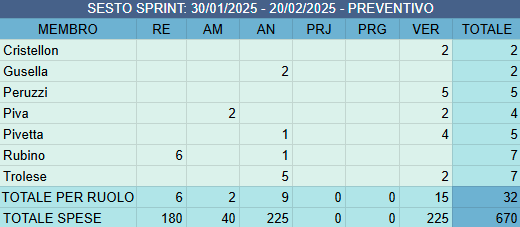
\includegraphics[width=0.6\linewidth]{preventivoOreSestoSprint.PNG}
    	\caption{Preventivo orario per membro - Sesto sprint}
    	\label{fig:Preventivo orario per membro - Sesto sprint}
    \end{figure}

    \begin{figure}[H]
        \centering
        \begin{tikzpicture}
            \pie[
                text=pin,
                hide number,
                color={responsabile, amministratore, analista, verificatore}, 
                radius=1.5
            ]{19/Responsabile - 19\%, 6/Amministratore - 6\%, 28/Analista - 28\% , 47/Verificatore - 47\%}
        \end{tikzpicture}
        \caption{Diagramma circolare della partizione delle ore preventive per ruolo - Sesto sprint }
        \label{fig:Diagramma circolare della partizione delle ore preventive per ruolo - Sesto sprint}
    \end{figure}
    
    \paragraph{Consuntivo orario}\mbox{}\vspace{0.4em}
    \begin{figure}[ht]
    	\centering
    	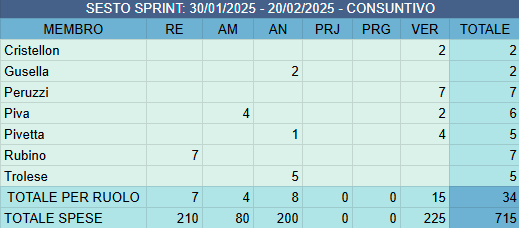
\includegraphics[width=0.6\linewidth]{consuntivoOreSestoSprint.png}
    	\caption{Consuntivo orario per membro - Sesto sprint}
    	\label{fig:Consuntivo orario per membro - Sesto sprint}
    \end{figure}

    \begin{figure}[H]
        \centering
        \begin{tikzpicture}
            \pie[
                text=pin,
                hide number,
                color={responsabile, amministratore, analista, verificatore}, 
                radius=1.5
            ]{21/Responsabile - 21\%, 12/Amministratore - 12\%, 23/Analista - 23\% , 44/Verificatore - 44\%}
        \end{tikzpicture}
        \caption{Diagramma circolare della partizione delle ore consuntive per ruolo - Sesto sprint }
        \label{fig:Diagramma circolare della partizione delle ore consuntive per ruolo - Sesto sprint}
    \end{figure}

    \paragraph{Rendicontazione delle risorse economiche restanti}\mbox{}\vspace{0.4em}
    \begin{figure}[H]
    	\centering
    	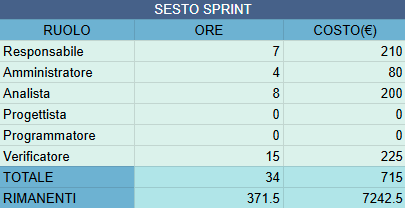
\includegraphics[width=0.6\linewidth]{oreCostiSestoSprint.png}
    	\caption{Consuntivo orario e costi per ruolo - Sesto sprint}
    	\label{fig:Consuntivo orario e costi per ruolo - Sesto sprint}
    \end{figure}
    
    \paragraph{Retrospettiva}\mbox{}\vspace{0.4em}

    Durante il sesto periodo si è svolta la prima parte della revisione RTB$_G$ con il professor Cardin, ottenendo un esito positivo e il semaforo verde. A seguito della revisione, il professore ha evidenziato alcune criticità nell’Analisi dei Requisiti, per le quali sono già state avviate le opportune attività correttive.
    Analogamente al quinto sprint$_G$, anche questo periodo è stato influenzato dalla sessione d’esami universitari, che ha ridotto la disponibilità dei membri del gruppo e rallentato il completamento di alcune attività. Nonostante ciò, il team ha mantenuto un impegno costante per concludere la documentazione$_G$ necessaria e integrare le modifiche richieste.
    Oltre alla revisione dei documenti, è stato portato avanti il lavoro sulle metriche e sul Piano di Qualifica, con un focus particolare sul cruscotto$_G$ e sulla validazione dei test$_G$. L’analisi dei dati emersi ha permesso di individuare alcuni aspetti migliorabili nella gestione della qualità, che verranno affrontati nei prossimi sprint$_G$.
    Infine, il confronto con l’azienda ha permesso di chiarire alcuni aspetti critici e pianificare le attività rimanenti. L’obiettivo del prossimo sprint$_G$ sarà consolidare le correzioni richieste e prepararsi alla seconda parte della revisione RTB$_G$, garantendo la massima aderenza agli standard qualitativi stabiliti.
    A seguito del termine della sessione d'esami per tutti i membri del team, il gruppo aumenterà il numero di ore lavorative e, di conseguenza, la produttività nei prossimi sprint$_G$. Questo impegno aggiuntivo è finalizzato a rispettare quanto più possibile la nuova data di consegna del progetto$_G$, stabilita dal gruppo per il 04-04-2025.
    
    %%%%%%%%%%
    %%%%% Settimo sprint
    %%%%%%%%%%%

    \newpage
    \subsubsection{Settimo sprint}
    \label{settimo-sprint}
        
        \paragraph{Durata sprint}\mbox{}\\
        \vspace{-1.5em}
        \begin{table}[h] 
        \renewcommand{\arraystretch}{1.2}  
        \begin{tabular}{ l l }
            Inizio: & 2025-02-21 \\
            Fine Prevista: & 2025-03-06 \\
            Fine Effettiva: & 2025-03-06 \\
            Giorni di ritardo: & 0 \\
        \end{tabular}
        \end{table}
        \vspace{-2em}
        {\renewcommand{\arraystretch}{1.5}%
        
        \paragraph{Panoramica generale e obiettivi}\mbox{}\vspace{0.4em}

        Nel corso del settimo sprint$_G$ il gruppo si propone di ultimare la consegna RTB$_G$ tramite il colloquio conclusivo con il professor 
        Vardanega, e di procedere con la fase di progettazione e sviluppo del MVP$_G$.
        \\
        Il gruppo ha in programma di:
        \begin{itemize}
            \item Concludere la revisione RTB$_G$, in un incontro con il professor Vardanega programmato per lunedì 2025-02-25 dalle 18:30 alle 18:50;
            \item Organizzare un incontro con il proponente$_G$ sullo stato avanzamento lavori;
            \item Iniziare la fase di progettazione del prodotto MVP$_G$.
        \end{itemize}

        Seguono le attività inserite nel backlog per questo periodo:
        \vspace{-0.5em}
        \begin{itemize}
        \setlength\itemsep{-0.2em}
        \item [-] Inizio stesura documento specifica tecnica;
        \item [-] Inizio stesura diagrammi delle classi;
        \item [-] Automatizzazione dell'esecuzione dei test$_G$ di unità in un ottica di Continuous-integration$_G$;
        \item [-] Implementazione della simulazione sensori con multithreading;
        \item [-] Implementazione dei test$_G$ automatizzati.
        \end{itemize}

        \paragraph{Gestione Rischi}\mbox{}
        \vspace{-1em}
        \subparagraph*{Rischi Attesi}\mbox{}
        
        Relativamente alla settima iterazione sono stati identificati dei potenziali rischi in cui potrebbe imbattersi il gruppo:
        \vspace{-0.5em}
        \begin{itemize}
        \setlength\itemsep{-0.2em}
        \item [-] \hyperref[RT3]{RT3} - Produzione di codice confuso o con errori;
        \item [-] \hyperref[RP1]{RP1} - Indisponibilità individuale o malattia;
        \item [-] \hyperref[RP2]{RP2} - Incertezza sulle stime delle attività.
        \end{itemize}

        \subparagraph*{Rischi Incontrati}\mbox{}
        
        Durante il settimo periodo il gruppo si è imbattuto in diversi rischi, fra i quali l'indisponibilità di uno dei membri del team a causa di malattia, e una serie
        di difficoltà legate alla fase di progettazione del prodotto, affrontata per la prima volta dal team. Nello specifico, la scarsa esperienza del gruppo in ambito 
        progettuale, ha reso difficile la definizione di un adeguato livello di complessità e granularità del design, che si è tradotta nella scrittura di codice confuso
        e con errori. Inoltre l'inesperienza del team ha reso difficile la stima delle attività.       

        \paragraph{Definizione ruoli}\mbox{}\vspace{0.4em}
        
        Questi sono i ruoli assegnati per membro in questo settimo sprint$_G$.\\
        \begin{table}[H]
            \centering
            \begin{tabular}{|c|c|}
            \hline
            \rowcolor{gray!25}
            \textbf{Ruolo} & \textbf{Membro}\\
            \hline
            Responsabile & Giovanni Cristellon \\
            \hline
            Progettista & Leonardo Trolese \\
            & Uncas Peruzzi\\
            & Alfredo Rubino\\
            \hline
            Programmatore & Federico Pivetta\\
            \hline
            Verificatore & Manuel Gusella \\
            & Riccardo Piva\\
            \hline
            \end{tabular}
            \caption{Tabella dei ruoli - Settimo Sprint}
        \end{table}

        \paragraph{Preventivo orario}\mbox{}\vspace{0.4em}
        \begin{figure}[H]
            \centering
            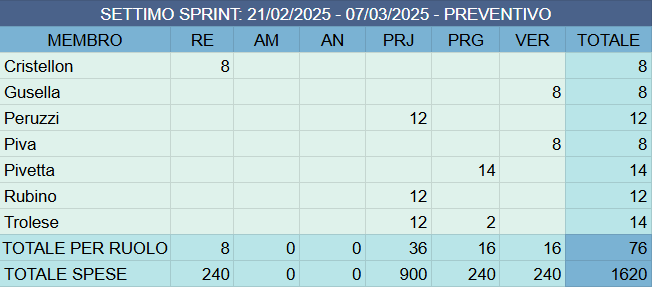
\includegraphics[width=0.6\linewidth]{preventivoOreSettimoSprint.png}
            \caption{Preventivo orario per membro - Settimo sprint}
            \label{fig:Preventivo orario per membro - Settimo sprint}
        \end{figure}

        \begin{figure}[H]
            \centering
            \begin{tikzpicture}
                \pie[
                    text=pin,
                    hide number,
                    color={responsabile, verificatore, progettista, programmatore}, 
                    radius=1.5
                ]{11/Responsabile - 11\% , 21/Verificatore - 21\%, 47/Progettista - 47\%, 21/Programmatore - 21\%}
            \end{tikzpicture}
            \caption{Diagramma circolare della partizione delle ore preventive per ruolo - Settimo sprint }
            \label{fig:Diagramma circolare della partizione delle ore preventive per ruolo - Settimo sprint}
        \end{figure}
        
        \paragraph{Consuntivo orario}\mbox{}\vspace{0.4em}
        \begin{figure}[ht]
            \centering
            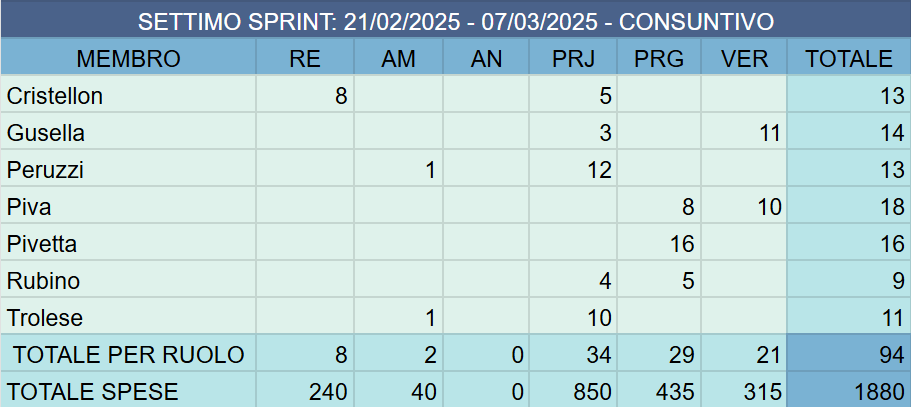
\includegraphics[width=0.6\linewidth]{consuntivoOreSettimoSprint.png}
            \caption{Consuntivo orario per membro - Settimo sprint}
            \label{fig:Consuntivo orario per membro - Settimo sprint}
        \end{figure}

        \begin{figure}[H]
            \centering
            \begin{tikzpicture}
                \pie[
                    text=pin,
                    hide number,
                    color={responsabile, amministratore, analista, verificatore, progettista, programmatore}, 
                    radius=1.5
                ]{9/Responsabile - 9\%, 2/Amministratore - 2\%, 22/Verificatore - 22\%, 36/Progettista - 36\%, 31/Programmatore - 31\%}
            \end{tikzpicture}
            \caption{Diagramma circolare della partizione delle ore consuntive per ruolo - Settimo sprint }
            \label{fig:Diagramma circolare della partizione delle ore consuntive per ruolo - Settimo sprint}
        \end{figure}

        \paragraph{Rendicontazione delle risorse economiche restanti}\mbox{}\vspace{0.4em}
        \begin{figure}[H]
            \centering
            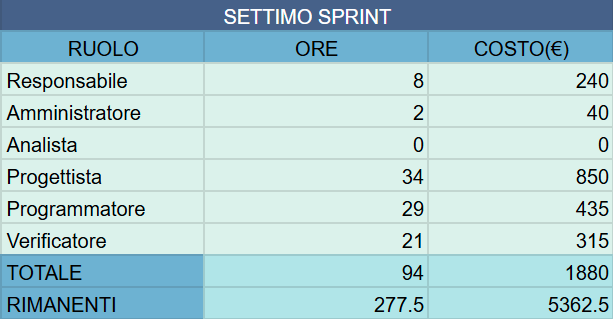
\includegraphics[width=0.6\linewidth]{oreCostiSettimoSprint.png}
            \caption{Consuntivo orario e costi per ruolo - Settimo sprint}
            \label{fig:Consuntivo orario e costi per ruolo - Settimo sprint}
        \end{figure}
        
        \paragraph{Retrospettiva}\mbox{}\vspace{0.4em}

        Durante il settimo periodo il gruppo ha affrontato il colloquio RTB$_G$ con il professor Vardanega, ottenendo un esito positivo. Inoltre ha avuto modo di 
        cimentarsi per la prima volta nella progettazione del prodotto.

        \subparagraph{Analisi delle strategie di mitigazione adottate}\mbox{}\vspace{0.4em}

        Come atteso, la fase di progettazione ha presentato alcune difficoltà, che erano però già state individuate in fase di analisi dei rischi. Questo ha permesso
        al gruppo di adottare le strategie di mitigazione precedentemente individuate. Nello specifico, per affrontare il rischio$_G$ RP2 (incertezza sulle stime delle 
        attività), il gruppo avrebbe dovuto introdurre un margine di sicurezza nelle stime orarie effettuate a inizio sprint$_G$; tuttavia ciò non è stato fatto, e questo
        spiega la significativa differenza fra le ore stimate e quelle effettivamente consumate.\\ 
        Inoltre, il gruppo ha affrontato il rischio$_G$ RP1 (indisponibilità individuale o malattia), che non ha avuto però un impatto significativo sullo sprint$_G$ in 
        quanto il membri sono comunque riusciti a coordinarsi, riassegnando i compiti in modo da non influire sulle tempistiche.\\
        Il team ha infine affrontato il rischio$_G$ RT3 (produzione di codice confuso o con errori), adottando una strategia di cooperazione con brevi sedute di 
        peer-programming per garantire una buona comprensione da parte di tutti i componenti del codice prodotto. Sempre per mitigare il rischio$_G$ RT3, è inoltre stato 
        richiesto un colloquio con il professore Cardin per l'iterazione successiva.
        
        \subparagraph{Raffinamento delle stime}\mbox{}\vspace{0.4em}

        Basandosi su quanto prodotto nel settimo sprint$_G$ il gruppo può affermare di essere attualmente in linea (anzi leggermente in anticipo) rispetto alle stime originali.
        Il budget totale stimato per il completamento del progetto$_G$ è di 12.454,70€, rispetto ai 12.950,00€ inizialmente preventivati. Di questa cifra, 4.867,20€ 
        rappresentano i costi ancora da sostenere per completare il prodotto e la relativa documentazione$_G$.\\
        Questo è un indicatore positivo per il gruppo, che può confermare la consegna PB$_G$ del progetto$_G$ indicativamente per la data 2025-04-04, riprogrammata a seguito della 
        revisione RTB$_G$.\\
        Resta tuttavia aperto il problema dell'imprecisione nella stima delle ore di lavoro previste per ogni sprint$_G$, che anche in questa iterazione si è rivelata essere
        imprecisa.\\


    %%%%%%%%%%
    %%%%% Ottavo sprint
    %%%%%%%%%%%

    \newpage
    \subsubsection{Ottavo sprint}
    \label{ottavo-sprint}
        
        \paragraph{Durata sprint}\mbox{}\\
        \vspace{-1.5em}
        \begin{table}[h] 
        \renewcommand{\arraystretch}{1.2}  
        \begin{tabular}{ l l }
            Inizio: & 2025-03-10 \\
            Fine Prevista: & 2025-03-16 \\
            Fine Effettiva: & 2025-03-16 \\
            Giorni di ritardo: & 0 \\
        \end{tabular}
        \end{table}
        \vspace{-2em}
        {\renewcommand{\arraystretch}{1.5}%
        
        \paragraph{Panoramica generale e obiettivi}\mbox{}\vspace{0.4em}

        Nel corso dell'ottavo sprint$_G$ il gruppo si propone di proseguire con lo sviluppo del prodotto MVP$_G$, cercare di ultimare il diagramma delle classi e continuare con la redazione dei documenti.
        \\
        Il gruppo ha in programma di:
        \begin{itemize}
            \item Procedere con lo sviluppo del prodotto MVP$_G$;
            \item Cercare di ultimare il diagramma delle classi;
            \item Continuare con la stesura della Specifica Tecnica;
            \item Continuare con la stesura del Manuale-utente$_G$;
            \item Svolgere incontro con professor Cardin per chiarimenti riguardanti la progettazione.
        \end{itemize}

        Seguono le attività inserite nel backlog per questo periodo:
        \vspace{-0.5em}
        \begin{itemize}
        \setlength\itemsep{-0.2em}
        \item [-] Continuazione stesura documento Specifica Tecnica;
        \item [-] Continuazione stesura documento Manuale-utente$_G$;
        \item [-] Continuazione sviluppo prodotto MVP$_G$;
        \item [-] Svolto incontro con professor Cardin;
        \item [-] Correzione diagrammi delle classi in seguito all'incontro con il professor Cardin.
        \end{itemize}

        \paragraph{Gestione Rischi}\mbox{}
        \vspace{-1em}
        \subparagraph*{Rischi Attesi}\mbox{}
        
        Relativamente all'ottava iterazione, dato il proseguimento nello sviluppo del prodotto MVP$_G$ e la conseguente produzione di codice, il gruppo ha identificato alcuni potenziali rischi in cui potrebbe imbattersi:
        \vspace{-0.5em}
        \begin{itemize}
        \setlength\itemsep{-0.2em}
        \item [-] \hyperref[RT3]{RT3} - Produzione di codice confuso o con errori;
        \end{itemize}

        \subparagraph*{Rischi Incontrati}\mbox{}
        
        Durante questa settimana il gruppo non ha incontrato alcun rischio$_G$ maggiore.

        \paragraph{Definizione ruoli}\mbox{}\vspace{0.4em}
        
        Questi sono i ruoli assegnati per membro in questo ottavo sprint$_G$.\\
        \begin{table}[H]
            \centering
            \begin{tabular}{|c|c|}
            \hline
            \rowcolor{gray!25}
            \textbf{Ruolo} & \textbf{Membro}\\
            \hline
            Responsabile & Riccardo Piva \\
            \hline
            Progettista & Federico Pivetta \\
            & Manuel Gusella \\
            \hline
            Programmatore & Uncas Peruzzi \\
            & Giovanni Cristellon \\
            \hline
            Verificatore & Leonardo Trolese \\
            & Alfredo Rubino \\
            \hline
            \end{tabular}
            \caption{Tabella dei ruoli - Ottavo Sprint}
        \end{table}

        \paragraph{Preventivo orario}\mbox{}\vspace{0.4em}
        \begin{figure}[H]
            \centering
            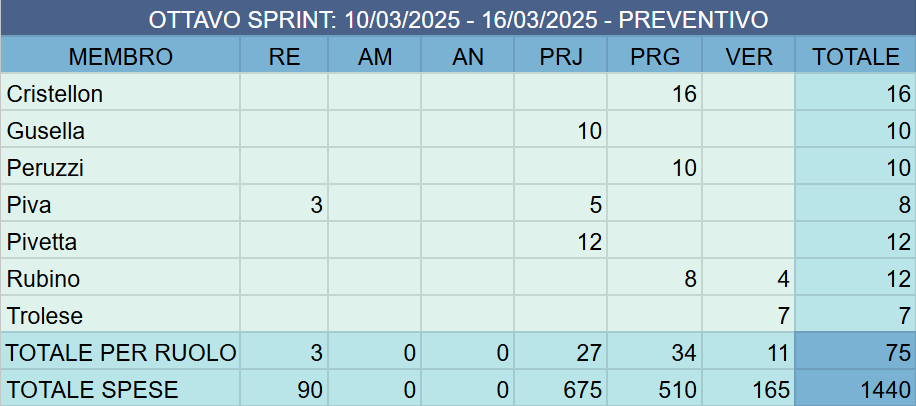
\includegraphics[width=0.6\linewidth]{preventivoOreOttavoSprint.png}
            \caption{Preventivo orario per membro - Ottavo sprint}
            \label{fig:Preventivo orario per membro - Ottavo sprint}
        \end{figure}

        \begin{figure}[H]
            \centering
            \begin{tikzpicture}
                \pie[
                    text=pin,
                    hide number,
                    color={responsabile, verificatore, progettista, programmatore}, 
                    radius=1.5
                ]{4/Responsabile - 4\% , 15/Verificatore - 15\%, 36/Progettista - 36\%, 45/Programmatore - 45\%}
            \end{tikzpicture}
            \caption{Diagramma circolare della partizione delle ore preventive per ruolo - Ottavo sprint}
            \label{fig:Diagramma circolare della partizione delle ore preventive per ruolo - Ottavo sprint}
        \end{figure}
        
        \paragraph{Consuntivo orario}\mbox{}\vspace{0.4em}
        \begin{figure}[ht]
            \centering
            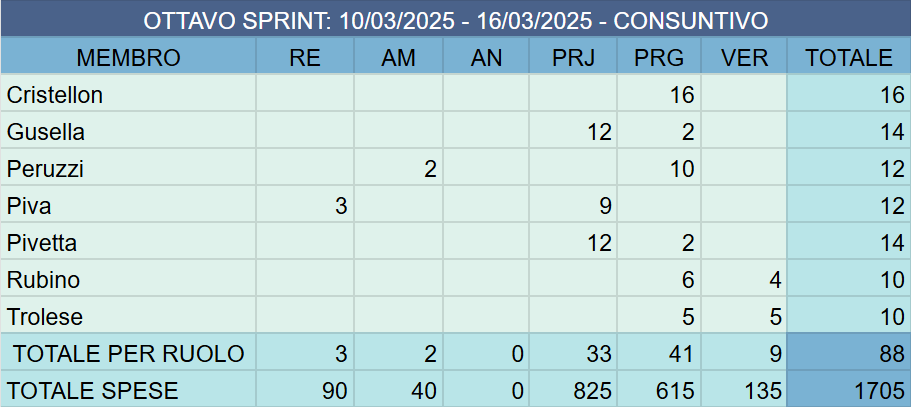
\includegraphics[width=0.6\linewidth]{consuntivoOreOttavoSprint.png}
            \caption{Consuntivo orario per membro - Ottavo sprint}
            \label{fig:Consuntivo orario per membro - Ottavo sprint}
        \end{figure}

        \begin{figure}[H]
            \centering
            \begin{tikzpicture}
                \pie[
                    text=pin,
                    hide number,
                    color={responsabile, amministratore, verificatore, progettista, programmatore}, 
                    radius=1.5
                ]{3/Responsabile - 3\%, 2/Amministratore - 2\%, 10/Verificatore - 10\%, 38/Progettista - 38\%, 47/Programmatore - 47\%}
            \end{tikzpicture}
            \caption{Diagramma circolare della partizione delle ore consuntive per ruolo - Ottavo sprint}
            \label{fig:Diagramma circolare della partizione delle ore consuntive per ruolo - Ottavo sprint}
        \end{figure}

        \paragraph{Rendicontazione delle risorse economiche restanti}\mbox{}\vspace{0.4em}
        \begin{figure}[H]
            \centering
            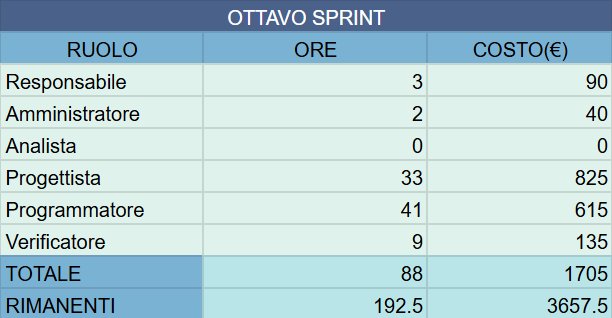
\includegraphics[width=0.6\linewidth]{oreCostiOttavoSprint.png}
            \caption{Consuntivo orario e costi per ruolo - Ottavo sprint}
            \label{fig:Consuntivo orario e costi per ruolo - Ottavo sprint}
        \end{figure}
        
        \paragraph{Retrospettiva}\mbox{}\vspace{0.4em}

        Durante l'ottavo periodo il gruppo ha effettuato una riunione con il professor Cardin per ricevere chiarimenti riguardanti la progettazione del prodotto MVP$_G$.
        Ha inoltre continuato con la fase di programmazione e con l'implementazione dei test$_G$ automatizzati.\\

        \subparagraph{Analisi delle strategie di mitigazione adottate}\mbox{}\vspace{0.4em}

        L'unico problema in cui il gruppo si è imbattuto è stato un errore nella progettazione sorto durante l'incontro con il professor Cardin.
        Grazie all'incremento delle ore produttive per sprint$_G$, dovuto anche al decremento della durata degli sprint$_G$ da due a una settimana, il gruppo è stato in grado di correggere l'errore in tempo e proseguire con lo sviluppo del prodotto$_G$.

        \subparagraph{Raffinamento delle stime}\mbox{}\vspace{0.4em}

        In base alle metriche aggiornate all'ottavo periodo il gruppo può dire di essere lievemente in anticipo.
        In base a quanto prodotto fin ora il budget totale stimato per il completamento del progetto$_G$ è di 12.616,96€, rispetto ai 12.950,00€ inizialmente prestabiliti.
        Di questa cifra, 3.324,40€ rappresentano i costi ancora da sostenere per completare il prodotto e la relativa documentazione$_G$.\\
        Questo è un buon segnale per il gruppo, facendo presagire che la consegna PB$_G$ stimata per il 2025-04-04 sia un obbiettivo raggiungibile.

    %%%%%%%%%%
    %%%%% Nono sprint
    %%%%%%%%%%%

    \newpage
    \subsubsection{Nono sprint}
    \label{nono-sprint}

    \paragraph{Durata sprint}\mbox{}\\
        \vspace{-1.5em}
        \begin{table}[h] 
        \renewcommand{\arraystretch}{1.2}  
        \begin{tabular}{ l l }
            Inizio: & 2025-03-17 \\
            Fine Prevista: & 2025-03-23 \\
            Fine Effettiva: & 2025-03-23 \\
            Giorni di ritardo: & 0 \\
        \end{tabular}
        \end{table}
        \vspace{-2em}
        {\renewcommand{\arraystretch}{1.5}%
        
        \paragraph{Panoramica generale e obiettivi}\mbox{}\vspace{0.4em}
        
        Nel corso del nono sprint$_G$, il gruppo si propone di proseguire con lo sviluppo del prodotto MVP$_G$ e dei relativi test$_G$ automatizzati, di rifinire ulteriormente la struttura del diagramma delle classi, avvicinandosi alla sua versione definitiva, e di continuare la redazione dei documenti.\\
        Il gruppo ha in programma di:
        \begin{itemize}
            \item Proseguire con lo sviluppo del prodotto MVP$_G$;
            \item Rifinire ulteriormente la struttura del diagramma delle classi;
            \item Continuare la stesura della documentazione$_G$ in vista della revisione PB$_G$;
            \item Definire ulteriori test$_G$ automatizzati;
            \item Finire di apportare le correzioni evidenziate nella revisione RTB$_G$ al documento \textit{Analisi\_dei\_Requisiti}.
        \end{itemize}
        Segue l'elenco delle attività inserite nel backlog per questa iterazione:
        \vspace{-0.5em}
        \begin{itemize}
        \setlength\itemsep{-0.2em}
            \item [-] Continuazione dello sviluppo del prodotto MVP$_G$;
            \item [-] Prosecuzione della redazione dei documenti;
            \item [-] Continuazione della scrittura dei test$_G$ automatizzati;
            \item [-] Ulteriore affinamento del diagramma delle classi;
            \item [-] Finalizzazione delle correzioni al documento \textit{Analisi\_dei\_Requisiti}.
        \end{itemize}

        \paragraph{Gestione Rischi}\mbox{}
        \vspace{-1em}
        \subparagraph*{Rischi Attesi}\mbox{}
        
        Relativamente alla nona iterazione, il gruppo ha identificato un potenziale rischio$_G$ legato all'assenza di un membro per una parte del periodo. Questa situazione potrebbe influire sulla distribuzione del carico di lavoro e sul rispetto delle scadenze previste. Di conseguenza, il gruppo ha individuato il seguente rischio$_G$:
        \vspace{-0.5em}
        \begin{itemize}
        \setlength\itemsep{-0.2em}
        \item [-] RP1 - Impegni al di fuori del progetto$_G$ o indisponibilità individuale.
        \end{itemize}

        \subparagraph*{Rischi Incontrati}\mbox{}
        
        Nonostante il rischio$_G$ atteso, il gruppo è riuscito a gestire efficacemente le attività, redistribuendo il carico di lavoro e ottimizzando le risorse disponibili. Grazie a una buona organizzazione e collaborazione, tutte le attività previste sono state completate entro i tempi stabiliti.
        
        \paragraph{Definizione ruoli}\mbox{}\vspace{0.4em}
        
        Questi sono i ruoli assegnati per membro in questo nono sprint$_G$.\\
        \begin{table}[H]
            \centering
            \begin{tabular}{|c|c|}
            \hline
            \rowcolor{gray!25}
            \textbf{Ruolo} & \textbf{Membro}\\
            \hline
            Responsabile & Federico Pivetta \\
            \hline
            Amministratore & Giovanni Cristellon \\
            \hline
            Progettista & Riccardo Piva \\ & Leonardo Trolese \\ & Alfredo Rubino \\
            \hline
            Programmatore & Manuel Gusella \\
            \hline
            Verificatore & Uncas Peruzzi \\
            \hline
            \end{tabular}
            \caption{Tabella dei ruoli - Nono Sprint}
        \end{table}

        \paragraph{Preventivo orario}\mbox{}\vspace{0.4em}
        \begin{figure}[H]
            \centering
            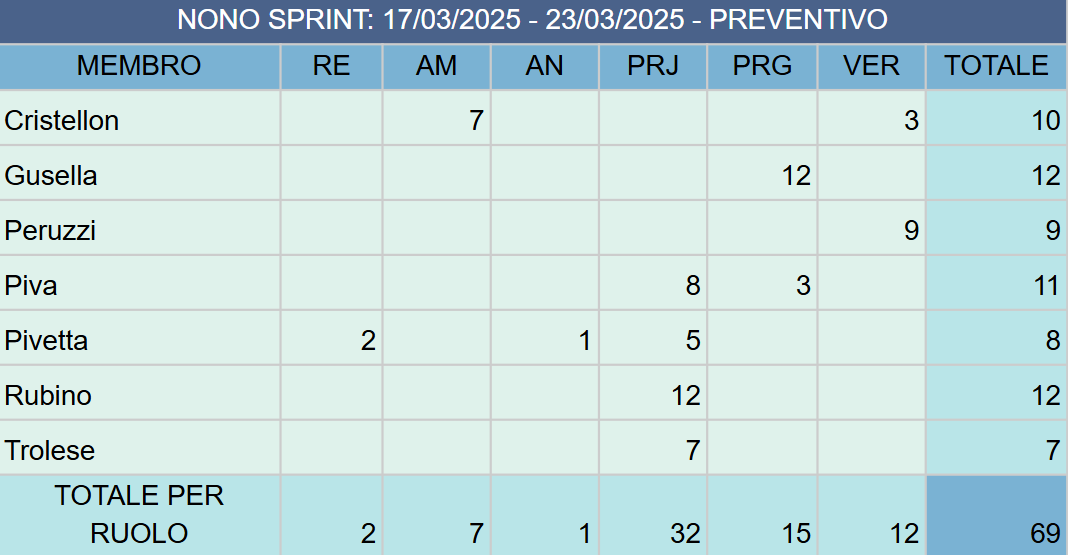
\includegraphics[width=0.6\linewidth]{preventivoOreNonoSprint.PNG}
            \caption{Preventivo orario per membro - Nono sprint}
            \label{fig:Preventivo orario per membro - Nono sprint}
        \end{figure}

        \begin{figure}[H]
            \centering
            \begin{tikzpicture}
                \pie[
                    text=pin,
                    hide number,
                    color={responsabile, verificatore, progettista, programmatore, amministratore, analista}, 
                    radius=1.5
                ]{3/Responsabile - 3\% , 10/Amministratore - 10\%, 1/Analista - 1\%,18/Verificatore - 18\%, 46/Progettista - 46\%, 22/Programmatore - 22\%}
            \end{tikzpicture}
            \caption{Diagramma circolare della partizione delle ore preventive per ruolo - Nono sprint}
            \label{fig:Diagramma circolare della partizione delle ore preventive per ruolo - Nono sprint}
        \end{figure}
        
        \paragraph{Consuntivo orario}\mbox{}\vspace{0.4em}
        \begin{figure}[ht]
            \centering
            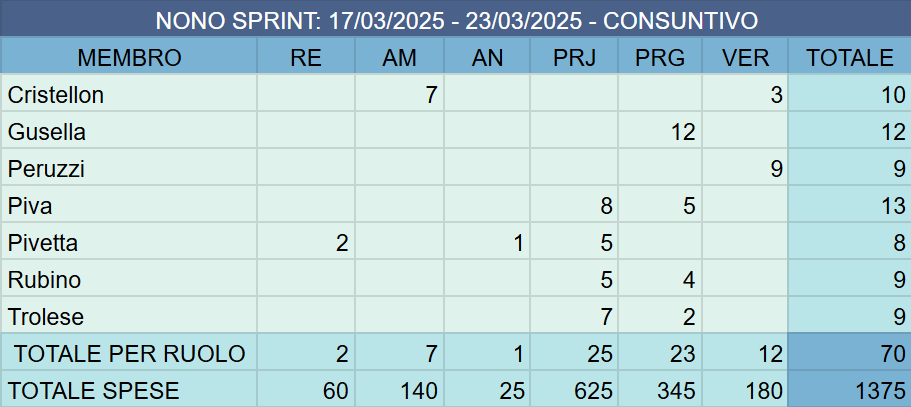
\includegraphics[width=0.6\linewidth]{consuntivoOreNonoSprint.PNG}
            \caption{Consuntivo orario per membro - Nono sprint}
            \label{fig:Consuntivo orario per membro - Nono sprint}
        \end{figure}

        \begin{figure}[H]
            \centering
            \begin{tikzpicture}
                \pie[
                    text=pin,
                    hide number,
                    color={responsabile, verificatore, progettista, programmatore, amministratore, analista}, 
                    radius=1.5
                ]{3/Responsabile - 3\%, 10/Amministratore - 10\%, 2/Analista - 2\%, 17/Verificatore - 17\%, 35/Progettista - 35\%, 33/Programmatore - 33\%}
            \end{tikzpicture}
            \caption{Diagramma circolare della partizione delle ore consuntive per ruolo - Nono sprint}
            \label{fig:Diagramma circolare della partizione delle ore consuntive per ruolo - Nono sprint}
        \end{figure}

        \paragraph{Rendicontazione delle risorse economiche restanti}\mbox{}\vspace{0.4em}
        \begin{figure}[H]
            \centering
            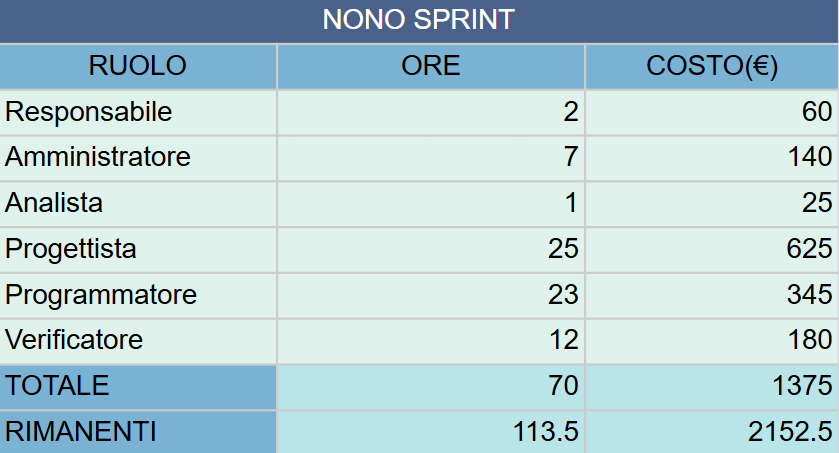
\includegraphics[width=0.6\linewidth]{oreCostiNonoSprint.png}
            \caption{Consuntivo orario e costi per ruolo - Nono sprint}
            \label{fig:Consuntivo orario e costi per ruolo - Nono sprint}
        \end{figure}
        
        \paragraph{Retrospettiva}\mbox{}\vspace{0.4em}
        
        Durante il nono sprint$_G$, il gruppo ha proseguito con lo sviluppo del prodotto MVP$_G$, concentrandosi sulla correzione di alcune funzionalità e sulla fusione della parte di simulazione delle posizioni con quella di generazione dei messaggi, oltre all'implementazione di ulteriori test$_G$ automatizzati. È stata quasi completata la struttura definitiva del diagramma delle classi, avvicinandosi alla sua versione finale, e sono state apportate le ultime correzioni al documento \textit{Analisi\_dei\_Requisiti} in base ai feedback$_G$ ricevuti. Parallelamente, è proseguita la redazione della documentazione$_G$ in vista della revisione PB$_G$.

        \subparagraph{Analisi delle strategie di mitigazione adottate}\mbox{}\vspace{0.4em}
        
        L'assenza di un membro del gruppo per una parte dello sprint$_G$ rappresentava un potenziale rischio$_G$ per il rispetto delle scadenze. Tuttavia, il gruppo ha adottato strategie di mitigazione efficaci, tra cui la redistribuzione del carico di lavoro e una migliore pianificazione delle attività. Di conseguenza, l'impatto della parziale assenza è stato ridotto al minimo, permettendo il completamento di tutte le attività previste senza ritardi significativi.

        \subparagraph{Raffinamento delle stime}\mbox{}\vspace{0.4em}

        In base alle metriche aggiornate al nono sprint$_G$, il budget totale stimato per il completamento del progetto$_G$ è di 12.546,94€, rispetto ai 12.950,00€ inizialmente 
        prestabiliti. Di questa cifra, 1.879,44€ rappresentano i costi ancora da sostenere per completare il prodotto e la relativa documentazione$_G$.\\
        Questo trend positivo indica una gestione efficiente delle risorse e un controllo accurato dei costi. Il gruppo può quindi procedere con maggiore sicurezza 
        verso le fasi finali del progetto$_G$, mantenendo comunque alta l'attenzione sulla qualità del lavoro e sul rispetto delle scadenze.


        %%%%%%%%%%
        %%%%% Decimo sprint
        %%%%%%%%%%%
    
        \newpage
        \subsubsection{Decimo sprint}
        \label{decimo-sprint}
    
        \paragraph{Durata sprint}\mbox{}\\
            \vspace{-1.5em}
            \begin{table}[h] 
            \renewcommand{\arraystretch}{1.2}  
            \begin{tabular}{ l l }
                Inizio: & 2025-03-24 \\
                Fine Prevista: & 2025-03-30 \\
                Fine Effettiva: & 2025-03-30 \\
                Giorni di ritardo: & 0 \\
            \end{tabular}
            \end{table}
            \vspace{-2em}
            {\renewcommand{\arraystretch}{1.5}%
            
            \paragraph{Panoramica generale e obiettivi}\mbox{}\vspace{0.4em}
            Nel corso del decimo sprint$_G$, il gruppo si propone di terminare la codifica del prodotto MVP$_G$, inclusi i testi di integrazione e di sistema$_G$. Inoltre, dopo aver progettato il diagramma della classi nella sua versione definitiva, l'obiettivo sarà terminare i documenti di \textit{Specifica\_Tecnica} e \textit{Manuale\_Utente} per poi preparare la presentazione necessaria alla revisione PB$_G$.
            Il gruppo ha in programma di:
            \begin{itemize}
                \item Terminare lo sviluppo dell'MVP;
                \item Terminare la scrittura dei documenti \textit{Specifica\_Tecnica} e \textit{Manuale\_Utente};
                \item Proseguire con la rifinitura degli altri documenti visto l'avvicinamento della data di consegna.
            \end{itemize}
            Segue l'elenco delle attività inserite nel backlog per questa iterazione:
            \vspace{-0.5em}
            \begin{itemize}
            \setlength\itemsep{-0.2em}
                \item [-] Verifica Finale Codice Repository$_G$;
                \item [-] Verifica rispetto Standard PEP8;
                \item [-] Verifica Finale Documento \textit{Specifica\_Tecnica};
                \item [-] Verifica Finale Documento \textit{Manuale\_Utente};
                \item [-] Redazione Presentazione per Product Baseline$_G$, revisione Cardin.
            \end{itemize}
    
            \paragraph{Gestione Rischi}\mbox{}
            \vspace{-1em}
            \subparagraph*{Rischi Attesi}\mbox{}
            
            Relativamente alla decima iterazione, il gruppo ha identificato un potenziale rischio$_G$ legato ad eventuali cambiamenti improvvisi a ridosso della consegna della Product Baseline$_G$. Questo a causa di errori che richiedono dei cambiamenti e una revisione delle attività già svolte oppure dovuto a incomprensioni tra i membri del team su alcune task.
            \vspace{-0.5em}
            \begin{itemize}
            \setlength\itemsep{-0.2em}
            \item [-]  RP3 - Cambiamenti improvvisi a ridosso della consegna.
            \end{itemize}
    
            \subparagraph*{Rischi Incontrati}\mbox{}
            Durante la decima iterazione, il rischio$_G$ di cambiamenti improvvisi a ridosso della consegna si è verificato a causa di un'incomprensione tra i membri del team riguardo al significato di una specifica task. Questo ha comportato la necessità di modificare una piccola parte della business logic di un servizio dell'MVP, con conseguenti revisioni delle attività già svolte, ma vista la mole della task, nessun rischio$_G$ di ritardo di consegna significativo.
            
            
            \paragraph{Definizione ruoli}\mbox{}\vspace{0.4em}
            
            Questi sono i ruoli assegnati per membro in questo decimo sprint$_G$.\\
            \begin{table}[H]
                \centering
                \begin{tabular}{|c|c|}
                \hline
                \rowcolor{gray!25}
                \textbf{Ruolo} & \textbf{Membro}\\
                \hline
                Responsabile & Uncas Peruzzi \\
                \hline
                Amministratore & Manuel Gusella \\
                \hline
                Progettista & Giovanni Cristellon \\
                \hline
                Programmatore & Leonardo Trolese \\ & Alfredo Rubino \\
                \hline
                Verificatore & Riccardo Piva\\ & Federico Pivetta \\
                \hline
                \end{tabular}
                \caption{Tabella dei ruoli - Decimo Sprint}
            \end{table}
    
            \paragraph{Preventivo orario}\mbox{}\vspace{0.4em}
            \begin{figure}[H]
                \centering
                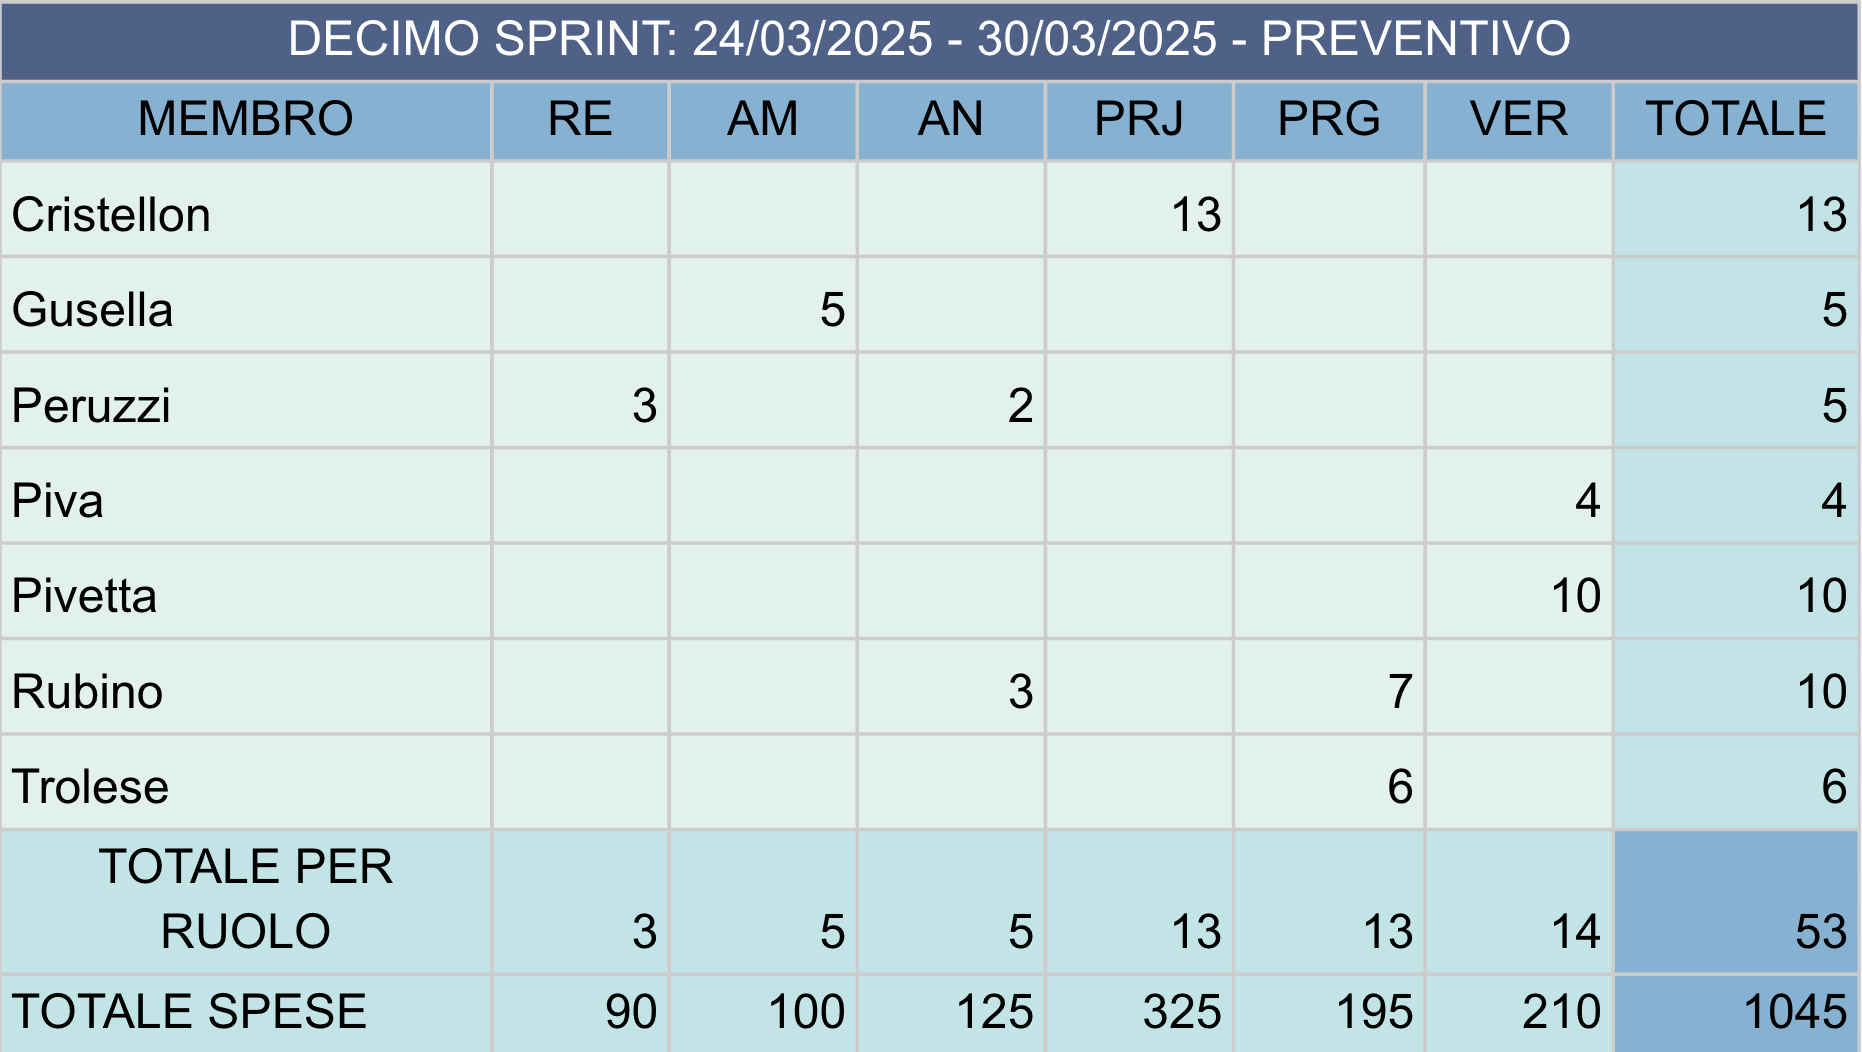
\includegraphics[width=0.6\linewidth]{preventivoOreDecimoSprint.PNG}
                \caption{Preventivo orario per membro - Decimo sprint}
                \label{fig:Preventivo orario per membro - Decimo sprint}
            \end{figure}
    
            \begin{figure}[H]
                \centering
                \begin{tikzpicture}
                    \pie[
                        text=pin,
                        hide number,
                        color={responsabile, verificatore, progettista, programmatore, amministratore, analista}, 
                        radius=1.5
                    ]{6/Responsabile - 6\% , 9/Amministratore - 9\%, 9/Analista - 9\%,26/Verificatore - 26\%, 25/Progettista - 25\%, 25/Programmatore - 25\%}
                \end{tikzpicture}
                \caption{Diagramma circolare della partizione delle ore preventive per ruolo - Decimo sprint}
                \label{fig:Diagramma circolare della partizione delle ore preventive per ruolo - Decimo sprint}
            \end{figure}
            
            \paragraph{Consuntivo orario}\mbox{}\vspace{0.4em}
            \begin{figure}[ht]
                \centering
                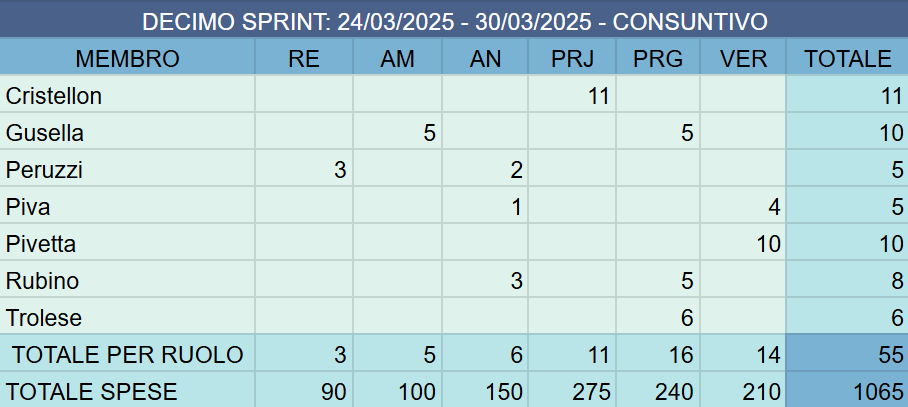
\includegraphics[width=0.6\linewidth]{consuntivoOreDecimoSprint.PNG}
                \caption{Consuntivo orario per membro - Decimo sprint}
                \label{fig:Consuntivo orario per membro - Decimo sprint}
            \end{figure}
    
            \begin{figure}[H]
                \centering
                \begin{tikzpicture}
                    \pie[
                        text=pin,
                        hide number,
                        color={responsabile, verificatore, progettista, programmatore, amministratore, analista}, 
                        radius=1.5
                    ]{5/Responsabile - 5\%, 9/Amministratore - 9\%, 11/Analista - 11\%, 26/Verificatore - 26\%, 20/Progettista - 20\%, 29/Programmatore - 29\%}
                \end{tikzpicture}
                \caption{Diagramma circolare della partizione delle ore consuntive per ruolo - Decimo sprint}
                \label{fig:Diagramma circolare della partizione delle ore consuntive per ruolo - Decimo sprint}
            \end{figure}
    
            \paragraph{Rendicontazione delle risorse economiche restanti}\mbox{}\vspace{0.4em}
            \begin{figure}[H]
                \centering
                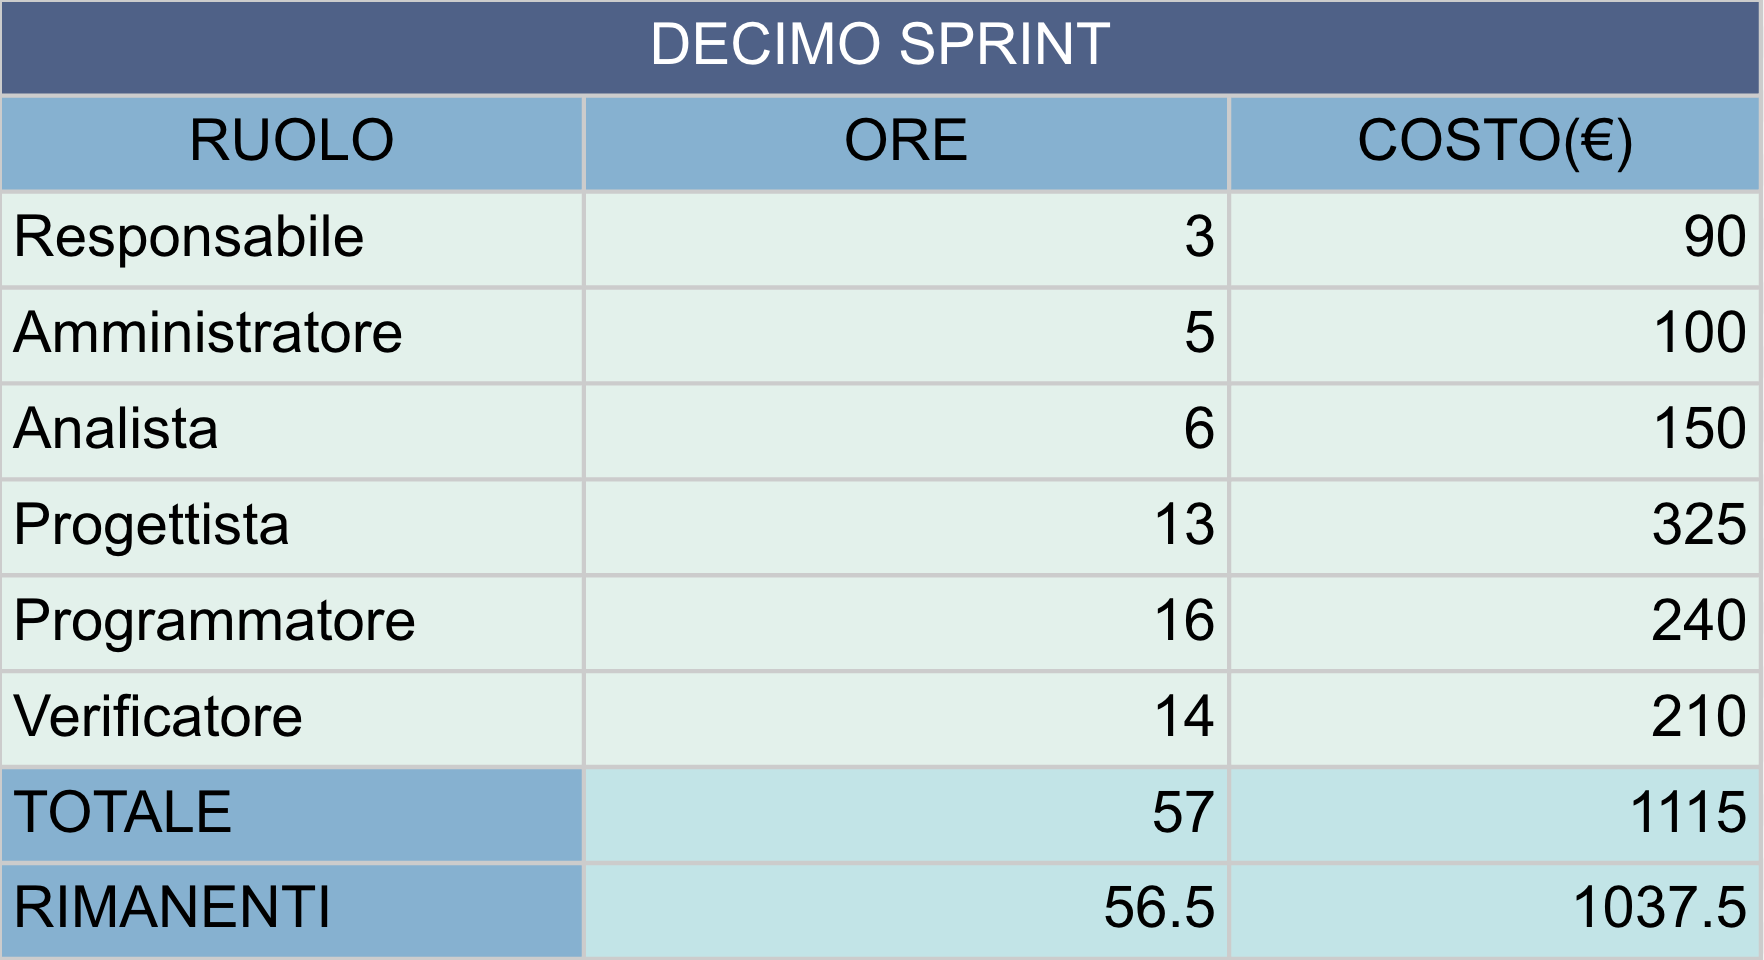
\includegraphics[width=0.6\linewidth]{oreCostiDecimoSprint.png}
                \caption{Consuntivo orario e costi per ruolo - Decimo sprint}
                \label{fig:Consuntivo orario e costi per ruolo - Decimo sprint}
            \end{figure}
            
            \paragraph{Retrospettiva}\mbox{}\vspace{0.4em}

            Durante il decimo sprint$_G$, il gruppo ha notato la fondamentale importanza di adottare una chiara comunicazione tra membri del team, soprattutto durante lo s
            viluppo del core del software. Trattandosi di una piccola modifica, non ha intaccato la data di consegna, ma potenzialmente avrebbe potuto creare problemi 
            di rilevanza maggiore. Sono stati inoltre terminati i documenti necessari alla revisione PB$_G$ con il Professor. Cardin, ed è stata iniziata la redazione 
            della presentazione necessaria al colloquio.
    
            \subparagraph{Analisi delle strategie di mitigazione adottate}\mbox{}\vspace{0.4em}
            
            Per mitigare il problema sorto, è stato necessario organizzare una piccola sessione di \textit{peer-to-peer programming} durante la quale i programmatori 
            hanno potuto chiarire e risolvere il problema presente nella business logic senza troppe difficoltà. Questo ha evidenziato come il lavoro sincrono, sebbene 
            più oneroso in termini di tempo e risorse, favorisca una maggiore produttività, in quanto facilita la comunicazione immediata, accelera la risoluzione dei 
            problemi e promuove una collaborazione più stretta tra i membri del team.
    
            \subparagraph{Raffinamento delle stime}\mbox{}\vspace{0.4em}
            
            Anche per il decimo periodo il gruppo può confermare il leggero anticipo rispetto alle stime originali già osservato nel corso delle iterazioni precedenti:
            nello specifico il budget stimato per il completamento del progetto$_G$ è di 12.666,59€, in leggero aumento rispetto allo sprint$_G$ precedente, ma comunque al di
            sotto del budget originale di 12.950,00€ inizialmente preventivato.\\
            Della cifra sopra citata, 934,10€ rappresentano i costi ancora da sostenere per completare il prodotto e la relativa documentazione$_G$.\\
            Questo è un indicatore positivo per il gruppo, che può riconfermare la consegna PB$_G$ del progetto$_G$ indicativamente per la data 2025-04-04, previa disponibilità 
            da parte dei professori.\\

        


        %%%%%%%%%%
        %%%%% Undicesimo sprint
        %%%%%%%%%%%
    
        \newpage
        \subsubsection{Undicesimo sprint}
        \label{undicesimo-sprint}
    
        \paragraph{Durata sprint}\mbox{}\\
            \vspace{-1.5em}
            \begin{table}[h] 
            \renewcommand{\arraystretch}{1.2}  
            \begin{tabular}{ l l }
                Inizio: & 2025-03-31 \\
                Fine Prevista: & 2025-04-06 \\
                Fine Effettiva: & 2025-04-11 \\
                Giorni di ritardo: & 5 \\
            \end{tabular}
            \end{table}
            \vspace{-2em}
            {\renewcommand{\arraystretch}{1.5}%
            
            \paragraph{Panoramica generale e obiettivi}\mbox{}\vspace{0.4em}
            Nel corso del decimo sprint$_G$, il gruppo si propone di effettuare la verifica conclusiva di tutta la documentazione$_G$ prodotta o modificata nel corso della 
            seconda fase del progetto$_G$, e di fissare e svolgere l'incontro con la proponente$_G$ Sync Lab per la presentazione del prodotto MVP$_G$; oltre che gli incontri di 
            revisione PB$_G$ con i professori Cardin e Vardanega.\\
            Il gruppo ha in programma di:
            \begin{itemize}
                \item Effettuare la verifica conclusiva della documentazione$_G$;
                \item Svolgere l'incontro con la proponente$_G$ Sync Lab per la presentazione del prodotto MVP$_G$;
                \item Svolgere gli incontri di revisione PB$_G$ con i professori Cardin e Vardanega.
            \end{itemize}
            Segue l'elenco delle attività inserite nel backlog per questa iterazione:
            \vspace{-0.5em}
            \begin{itemize}
            \setlength\itemsep{-0.2em}
                \item [-] Verifica Finale Documento \textit{Specifica\_Tecnica};
                \item [-] Verifica Finale Documento \textit{Manuale\_Utente};
                \item [-] Verifica Finale Documento \textit{Analisi\_dei\_Requisiti};
                \item [-] Analisi delle metriche nel documento \textit{Piano\_di\_Qualifica};
                \item [-] Correzione glossario;
                \item [-] Presentazione del prodotto MVP$_G$ alla proponente$_G$ Sync Lab;
                \item [-] Redazione Presentazione per Product Baseline$_G$, revisione Cardin;
                \item [-] Redazione Presentazione per Product Baseline$_G$, revisione Vardanega.
            \end{itemize}
    
            \paragraph{Gestione Rischi}\mbox{}
            \vspace{-1em}
            \subparagraph*{Rischi Attesi}\mbox{}
            
            Relativamente alla undicesima iterazione, il gruppo ha identificato il potenziale rischio$_G$ dovuto a cambiamenti improvvisi a ridosso della consegna PB$_G$ (RP3),
            come nel caso del decimo sprint$_G$; e il potenziale rischio$_G$ di incertezza nella stima delle attività (RP2), dovuto principalmente all'impossibilità di 
            prevedere con certezza i tempi di consegna (poiché direttamente influenzati dalla disponibilità dei professori Cardin e Vardanega).\\
            \vspace{-0.5em}
            \begin{itemize}
            \setlength\itemsep{-0.2em}
            \item [-]  RP2 - Incertezza nella stima delle attività;
            \item [-]  RP3 - Cambiamenti improvvisi a ridosso della consegna.
            \end{itemize}
    
            \subparagraph*{Rischi Incontrati}\mbox{}
            Durante la undicesima iterazione il rischio$_G$ RP3 si è verificato poiché il gruppo ha dovuto apportare delle minimali correzioni al prodotto MVP$_G$ a seguito 
            dei suggerimenti emersi nell'incontro con la proponente$_G$ Sync Lab, tuttavia tale rischio$_G$ non ha comportato ritardi significativi.\\
            Anche il rischio$_G$ RP2 si è verificato, poiché gli incontri con i professori Cardin e Vardanega hanno rispettato le tempistiche previste per la consegna della 
            documentazione$_G$ e del prodotto MVP$_G$.\\
            
            
            \paragraph{Definizione ruoli}\mbox{}\vspace{0.4em}
            
            Questi sono i ruoli assegnati per membro in questo undicesimo sprint$_G$.\\
            \begin{table}[H]
                \centering
                \begin{tabular}{|c|c|}
                \hline
                \rowcolor{gray!25}
                \textbf{Ruolo} & \textbf{Membro}\\
                \hline
                Responsabile & Leonardo Trolese \\
                \hline
                Amministratore & / \\
                \hline
                Progettista & Uncas Peruzzi \\ & Alfredo Rubino \\
                \hline
                Programmatore & Riccardo Piva \\ & Federico Pivetta\\
                \hline
                Verificatore & Manuel Gusella \\ & Giovanni Cristellon \\
                \hline
                \end{tabular}
                \caption{Tabella dei ruoli - Undicesimo Sprint}
            \end{table}
    
            \paragraph{Preventivo orario}\mbox{}\vspace{0.4em}
            \begin{figure}[H]
                \centering
                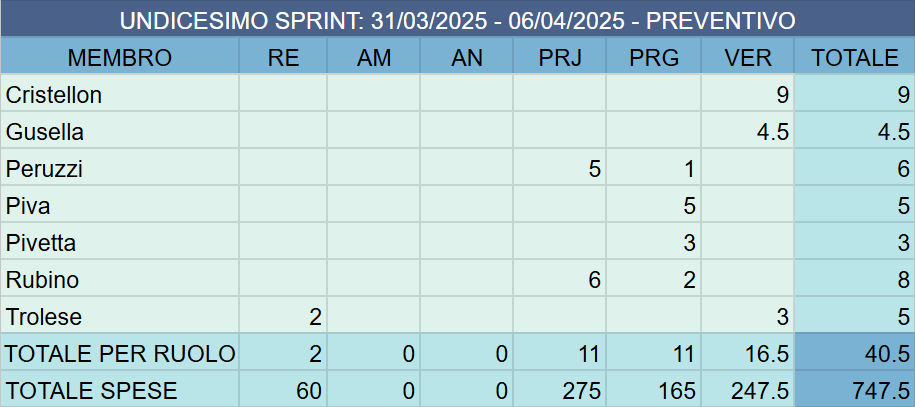
\includegraphics[width=0.6\linewidth]{preventivoOreUndicesimoSprint.PNG}
                \caption{Preventivo orario per membro - Undicesimo sprint}
                \label{fig:Preventivo orario per membro - Undicesimo sprint}
            \end{figure}
    
            \begin{figure}[H]
                \centering
                \begin{tikzpicture}
                    \pie[
                        text=pin,
                        hide number,
                        color={responsabile, amministratore, analista, verificatore, progettista, programmatore}, 
                        radius=1.5
                    ]{5/Responsabile - 5\%, 41/Verificatore - 41\%, 27/Progettista - 27\%, 27/Programmatore - 27\%}
                \end{tikzpicture}
                \caption{Diagramma circolare della partizione delle ore preventive per ruolo - Undicesimo sprint}
                \label{fig:Diagramma circolare della partizione delle ore preventive per ruolo - Undicesimo sprint}
            \end{figure}
            
            \paragraph{Consuntivo orario}\mbox{}\vspace{0.4em}
            \begin{figure}[ht]
                \centering
                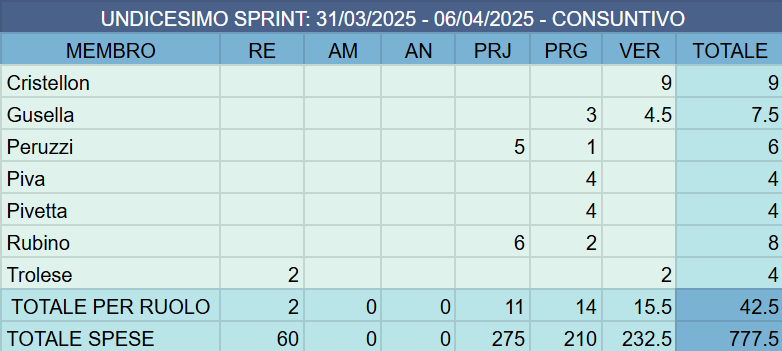
\includegraphics[width=0.6\linewidth]{consuntivoOreUndicesimoSprint.png}
                \caption{Consuntivo orario per membro - Undicesimo sprint}
                \label{fig:Consuntivo orario per membro - Undicesimo sprint}
            \end{figure}
    
            \begin{figure}[H]
                \centering
                \begin{tikzpicture}
                    \pie[
                        text=pin,
                        hide number,
                        color={responsabile, amministratore, analista, verificatore, progettista, programmatore}, 
                        radius=1.5
                        %TODO
                    ]{5/Responsabile - 5\%, 36/Verificatore - 36\%, 26/Progettista - 26\%, 33/Programmatore - 33\%}
                \end{tikzpicture}
                \caption{Diagramma circolare della partizione delle ore consuntive per ruolo - Undicesimo sprint}
                \label{fig:Diagramma circolare della partizione delle ore consuntive per ruolo - Undicesimo sprint}
            \end{figure}
    
            \paragraph{Rendicontazione delle risorse economiche restanti}\mbox{}\vspace{0.4em}
            \begin{figure}[H]
                \centering
                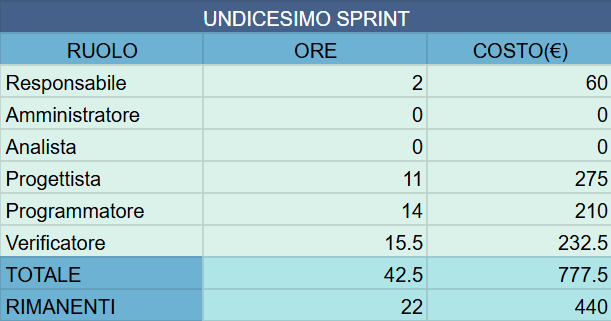
\includegraphics[width=0.6\linewidth]{oreCostiUndicesimoSprint.png}
                \caption{Consuntivo orario e costi per ruolo - Undicesimo sprint}
                \label{fig:Consuntivo orario e costi per ruolo - Undicesimo sprint}
            \end{figure}
            
            \paragraph{Retrospettiva}\mbox{}\vspace{0.4em}        
            Nel corso dell'undicesimo sprint$_G$ il gruppo, si è concentrato sulla produzione di documentazione$_G$ in preparazione alla revisione PB$_G$ avvenuta con il professor
            Cardin in data 2025-04-07. Sempre durante questo sprint$_G$ il gruppo ha anche sostenuto l'incontro di presentazione del prodotto MVP$_G$ con la proponente$_G$ Sync Lab,
            durante il quale sono stati presentati e approvati i risultati ottenuti fino a quel momento.\\
            A seguito di entrambi gli incontri c'è infine stato un periodo di conclusione della documentazione$_G$, in cui sono stati preparati i documenti necessari per la
            revisione PB$_G$ del professor Vardanega. Questo periodo ha costretto il gruppo ad allungare la durata dello sprint$_G$, e ciò ha confermato l'incorrere del rischio$_G$ 
            RP2 (incertezza nella stima delle attività) già previsto dal gruppo in fase di pianificazione.\\
    
            \subparagraph{Analisi delle strategie di mitigazione adottate}\mbox{}\vspace{0.4em}
            Il gruppo non ha dovuto mitigare in nessun modo il rischio$_G$ RP2, poiché i giorni di ritardo registrati non hanno comunque superato la data di ricezione dell'esito
            della revisione PB$_G$ del professor Cardin. Il gruppo può quindi affermare che tale ritardo non ha avuto alcun impatto sui tempi di consegne previsti.
    
            \subparagraph{Raffinamento delle stime}\mbox{}\vspace{0.4em}
            Il gruppo ha concluso il progetto$_G$ spendendo un totale di 12.510,00€, a fronte dei 12.950,00€ inizialmente preventivati in fase di redazione del preventivo 
            orario totale. Questo indica che il gruppo è riuscito a terminare il lavoro con un risparmio di 440,00€ rispetto al budget massimo spendibile. Il risultato
            ottenuto risulta quindi soddisfacente per il team, e in linea con le aspettative sorte in fase di realizzazione relativamente alla spesa totale.\\


\end{document}
